This section covers basic performance tests, i.e. how specific algorithms scale
with grid resolution and with polynomial degree, on a \emph{single compute node}.

% --------------------------------------------------------------------------------
\section{Solver Performance - Poisson/Stokes problems}
\label{sec:SolverPerformancePoisson}
% --------------------------------------------------------------------------------
Two groups of solver are compared:
\begin{itemize}
\item
Direct Solvers: directs sparse methods, such as PARDISO\footnote{
\url{http://www.pardiso-project.org/}}
and MUMPS\footnote{
\url{http://mumps.enseeiht.fr/}}
are compared.
Their performance also serves as a comparative baseline.

%\item
%Iterative Algorithms without preconditioning, resp. low-impact, generic preconditioning:
%This includes solver libraries such as \code{monkey} (BoSSS-specific, supports GPU)
%as well as
%HYPRE\footnote{
%\url{https://computation.llnl.gov/projects/hypre-scalable-linear-solvers-multigrid-methods}}
%(native library, used via wrappers).

\item
Iterative Algorithms with \ac{dg}-specific preconditioners, such as aggregation multigrid
and multi-level additive Schwarz
\end{itemize}

The scaling and performance is profiled subsequent sections. For Performance profiling we stick to our working horse: the kcycle-Schwarz algorithm (with optional p-two-grid as block solver).
The performance profile of the krylov V-cycle with Schwarz pre and post-smoother is investigated. A direct solver (PARDISO) is used to solve the deepest coarse system. One may choose another direct solver for the coarse system, e.g. MUMPS. In practise PARDISO is more robust to ill-conditioned system, therefore in this performance analysis investigation we will stick to PARDISO as solver, wherever a direct solver is needed.
NOTE: the p-two-grid used in Schwarz or as a standalone preconditioner, the coarse system is solved by a direct solver.

We distinguish four phases of every solver-scenario: 
\begin{itemize}
	\item MatrixAssembly: assemble Block matrix
	\item Aggregation basis init: create multigrid sequence, contains information about the transformation at the multigrid levels
	\item Solver Init: hand over/assemble relevant data for the chosen solver, e.g. operator matrix etc.
	\item Solver Run: solves the equation system: operator matrix, vector of dg coordinates and given RHS 
\end{itemize}
Matrix assembly and aggregation init is discritization specific, whereas, Solver init and run ist specific for the used solver.

\subsection{Introduction of solvers}

\subsubsection{linear Solver: p-two-grid}
\label{sec:ptg_gmres}

The p two grid algorithm can be used as left preconditioner for the well known GMRES-algorithm. Or as block solver of the Schwarz blocks in the Orthonormalization-multigrid algorithm, described in \ref{alg:OrthoMG}.

\subsubsection{linear Solver: V-krylov-cycle with Schwarz smoother}
\label{sec:kcycle}

The orthonormalization multigrid is a combination of a v-cycle of a geometric multigrid (or algebraic as the agglomeration of cells is graph based) with an additive Schwarz smoother and a projection method onto the history of residual contributions of parts of the algorithm (smoother and coarse grid correction). A schematic of the solver can be checked out in \ref{fig:SolverScheme}. 
For more details on the solvers check \cite{OpenSoftwarePDE}.

\begin{figure}[!h]
	\begin{center}
		\includegraphics[scale=0.65]{./apdx-NodeSolverPerformance/solver-scheme.png}
		\input{./apdx-NodeSolverPerformance/solver-scheme.png}
	\end{center}
	\caption{
		scheme of Orthonormalization Multigrid. The block solver is usually a direct solver like PARDISO. Note: for the smoother it is sufficient to solve the system approximately. This gives rise to approximate solutions of the Schwarz blocks, like a ILU algorithm.  
	}
	\label{fig:SolverScheme}
\end{figure}

\subsection{DG-Poisson test problem}
\label{sec:ConstantDiffusionCoefficient}
The stationary 3D-problem:
\begin{equation}
\left\{ \begin{array} {rclll}
- \Delta T   & = & g_{\domain}                      
& \text{in}\ \Omega = (0,10) \times (-1,1) \times (-1,1)  &  \\
% ----
T   & = & g_D = 0                             
& \text{on}\ \Gamma_D = \{ (x,y,z) \in \real^3; \ x = 0 \}
& \text{Dirichlet-boundary} \\
% ----
\nabla T \cdot \vec{n}_{\partial \domain} & = & g_N 
& \text{on}\ \Gamma_N = \partial \Omega \setminus \Gamma_D
& \text{Neumann-boundary}
\end{array} \right.
\label{eq:ContantCoeffPoissonBenchmark}
\end{equation}
where $g_{\domain}=-sin(x)$.
is investigated on a non-uniform, Cartesian grid
(equidistant in $z$, sinus-spacing in $x$ and $y$ direction).
The large $\Gamma_N$ makes the problem harder for non-preconditioned
iterative methods. See Figure \ref{fig:ConstantCoeffRuntimes} for results.

\subsection{DG-Poisson: scaling of solvers}

\graphicspath{{./apdx-NodeSolverPerformance/PoissonConstCoeff/plots/}}

\begin{figure}[!h]
	\begin{center}
		% GNUPLOT: LaTeX picture with Postscript
\begingroup
  \makeatletter
  \providecommand\color[2][]{%
    \GenericError{(gnuplot) \space\space\space\@spaces}{%
      Package color not loaded in conjunction with
      terminal option `colourtext'%
    }{See the gnuplot documentation for explanation.%
    }{Either use 'blacktext' in gnuplot or load the package
      color.sty in LaTeX.}%
    \renewcommand\color[2][]{}%
  }%
  \providecommand\includegraphics[2][]{%
    \GenericError{(gnuplot) \space\space\space\@spaces}{%
      Package graphicx or graphics not loaded%
    }{See the gnuplot documentation for explanation.%
    }{The gnuplot epslatex terminal needs graphicx.sty or graphics.sty.}%
    \renewcommand\includegraphics[2][]{}%
  }%
  \providecommand\rotatebox[2]{#2}%
  \@ifundefined{ifGPcolor}{%
    \newif\ifGPcolor
    \GPcolortrue
  }{}%
  \@ifundefined{ifGPblacktext}{%
    \newif\ifGPblacktext
    \GPblacktexttrue
  }{}%
  % define a \g@addto@macro without @ in the name:
  \let\gplgaddtomacro\g@addto@macro
  % define empty templates for all commands taking text:
  \gdef\gplbacktext{}%
  \gdef\gplfronttext{}%
  \makeatother
  \ifGPblacktext
    % no textcolor at all
    \def\colorrgb#1{}%
    \def\colorgray#1{}%
  \else
    % gray or color?
    \ifGPcolor
      \def\colorrgb#1{\color[rgb]{#1}}%
      \def\colorgray#1{\color[gray]{#1}}%
      \expandafter\def\csname LTw\endcsname{\color{white}}%
      \expandafter\def\csname LTb\endcsname{\color{black}}%
      \expandafter\def\csname LTa\endcsname{\color{black}}%
      \expandafter\def\csname LT0\endcsname{\color[rgb]{1,0,0}}%
      \expandafter\def\csname LT1\endcsname{\color[rgb]{0,1,0}}%
      \expandafter\def\csname LT2\endcsname{\color[rgb]{0,0,1}}%
      \expandafter\def\csname LT3\endcsname{\color[rgb]{1,0,1}}%
      \expandafter\def\csname LT4\endcsname{\color[rgb]{0,1,1}}%
      \expandafter\def\csname LT5\endcsname{\color[rgb]{1,1,0}}%
      \expandafter\def\csname LT6\endcsname{\color[rgb]{0,0,0}}%
      \expandafter\def\csname LT7\endcsname{\color[rgb]{1,0.3,0}}%
      \expandafter\def\csname LT8\endcsname{\color[rgb]{0.5,0.5,0.5}}%
    \else
      % gray
      \def\colorrgb#1{\color{black}}%
      \def\colorgray#1{\color[gray]{#1}}%
      \expandafter\def\csname LTw\endcsname{\color{white}}%
      \expandafter\def\csname LTb\endcsname{\color{black}}%
      \expandafter\def\csname LTa\endcsname{\color{black}}%
      \expandafter\def\csname LT0\endcsname{\color{black}}%
      \expandafter\def\csname LT1\endcsname{\color{black}}%
      \expandafter\def\csname LT2\endcsname{\color{black}}%
      \expandafter\def\csname LT3\endcsname{\color{black}}%
      \expandafter\def\csname LT4\endcsname{\color{black}}%
      \expandafter\def\csname LT5\endcsname{\color{black}}%
      \expandafter\def\csname LT6\endcsname{\color{black}}%
      \expandafter\def\csname LT7\endcsname{\color{black}}%
      \expandafter\def\csname LT8\endcsname{\color{black}}%
    \fi
  \fi
    \setlength{\unitlength}{0.0500bp}%
    \ifx\gptboxheight\undefined%
      \newlength{\gptboxheight}%
      \newlength{\gptboxwidth}%
      \newsavebox{\gptboxtext}%
    \fi%
    \setlength{\fboxrule}{0.5pt}%
    \setlength{\fboxsep}{1pt}%
\begin{picture}(7920.00,6800.00)%
    \gplgaddtomacro\gplbacktext{%
      \csname LTb\endcsname%
      \put(997,4825){\makebox(0,0)[r]{\strut{}$10^{-2}$}}%
      \csname LTb\endcsname%
      \put(997,5150){\makebox(0,0)[r]{\strut{}$10^{-1}$}}%
      \csname LTb\endcsname%
      \put(997,5475){\makebox(0,0)[r]{\strut{}$10^{0}$}}%
      \csname LTb\endcsname%
      \put(997,5800){\makebox(0,0)[r]{\strut{}$10^{1}$}}%
      \csname LTb\endcsname%
      \put(997,6126){\makebox(0,0)[r]{\strut{}$10^{2}$}}%
      \csname LTb\endcsname%
      \put(997,6451){\makebox(0,0)[r]{\strut{}$10^{3}$}}%
      \csname LTb\endcsname%
      \put(997,6776){\makebox(0,0)[r]{\strut{}$10^{4}$}}%
      \csname LTb\endcsname%
      \put(1099,4646){\makebox(0,0){\strut{} }}%
      \csname LTb\endcsname%
      \put(2137,4646){\makebox(0,0){\strut{} }}%
      \csname LTb\endcsname%
      \put(3176,4646){\makebox(0,0){\strut{} }}%
      \csname LTb\endcsname%
      \put(4214,4646){\makebox(0,0){\strut{} }}%
      \csname LTb\endcsname%
      \put(5252,4646){\makebox(0,0){\strut{} }}%
      \csname LTb\endcsname%
      \put(6291,4646){\makebox(0,0){\strut{} }}%
      \csname LTb\endcsname%
      \put(7329,4646){\makebox(0,0){\strut{} }}%
      \csname LTb\endcsname%
      \put(7431,4825){\makebox(0,0)[l]{\strut{} }}%
      \csname LTb\endcsname%
      \put(7431,5150){\makebox(0,0)[l]{\strut{} }}%
      \csname LTb\endcsname%
      \put(7431,5475){\makebox(0,0)[l]{\strut{} }}%
      \csname LTb\endcsname%
      \put(7431,5801){\makebox(0,0)[l]{\strut{} }}%
      \csname LTb\endcsname%
      \put(7431,6126){\makebox(0,0)[l]{\strut{} }}%
      \csname LTb\endcsname%
      \put(7431,6451){\makebox(0,0)[l]{\strut{} }}%
      \csname LTb\endcsname%
      \put(7431,6776){\makebox(0,0)[l]{\strut{} }}%
    }%
    \gplgaddtomacro\gplfronttext{%
      \csname LTb\endcsname%
      \put(397,5800){\rotatebox{-270}{\makebox(0,0){\strut{}$k = 2$}}}%
      \csname LTb\endcsname%
      \put(2190,6565){\makebox(0,0)[l]{\strut{}GMRES w. pTG}}%
      \csname LTb\endcsname%
      \put(2190,6286){\makebox(0,0)[l]{\strut{}Kcycle w. add.-Schwarz}}%
      \csname LTb\endcsname%
      \put(2190,6007){\makebox(0,0)[l]{\strut{}Pardiso}}%
      \csname LTb\endcsname%
      \put(2190,5728){\makebox(0,0)[l]{\strut{}linear}}%
    }%
    \gplgaddtomacro\gplbacktext{%
      \csname LTb\endcsname%
      \put(997,2558){\makebox(0,0)[r]{\strut{}$10^{-2}$}}%
      \csname LTb\endcsname%
      \put(997,2883){\makebox(0,0)[r]{\strut{}$10^{-1}$}}%
      \csname LTb\endcsname%
      \put(997,3209){\makebox(0,0)[r]{\strut{}$10^{0}$}}%
      \csname LTb\endcsname%
      \put(997,3534){\makebox(0,0)[r]{\strut{}$10^{1}$}}%
      \csname LTb\endcsname%
      \put(997,3859){\makebox(0,0)[r]{\strut{}$10^{2}$}}%
      \csname LTb\endcsname%
      \put(997,4185){\makebox(0,0)[r]{\strut{}$10^{3}$}}%
      \csname LTb\endcsname%
      \put(997,4510){\makebox(0,0)[r]{\strut{}$10^{4}$}}%
      \csname LTb\endcsname%
      \put(1099,2379){\makebox(0,0){\strut{} }}%
      \csname LTb\endcsname%
      \put(2137,2379){\makebox(0,0){\strut{} }}%
      \csname LTb\endcsname%
      \put(3176,2379){\makebox(0,0){\strut{} }}%
      \csname LTb\endcsname%
      \put(4214,2379){\makebox(0,0){\strut{} }}%
      \csname LTb\endcsname%
      \put(5252,2379){\makebox(0,0){\strut{} }}%
      \csname LTb\endcsname%
      \put(6291,2379){\makebox(0,0){\strut{} }}%
      \csname LTb\endcsname%
      \put(7329,2379){\makebox(0,0){\strut{} }}%
      \csname LTb\endcsname%
      \put(7431,2558){\makebox(0,0)[l]{\strut{} }}%
      \csname LTb\endcsname%
      \put(7431,2883){\makebox(0,0)[l]{\strut{} }}%
      \csname LTb\endcsname%
      \put(7431,3209){\makebox(0,0)[l]{\strut{} }}%
      \csname LTb\endcsname%
      \put(7431,3534){\makebox(0,0)[l]{\strut{} }}%
      \csname LTb\endcsname%
      \put(7431,3859){\makebox(0,0)[l]{\strut{} }}%
      \csname LTb\endcsname%
      \put(7431,4185){\makebox(0,0)[l]{\strut{} }}%
      \csname LTb\endcsname%
      \put(7431,4510){\makebox(0,0)[l]{\strut{} }}%
      \csname LTb\endcsname%
      \put(1099,4689){\makebox(0,0){\strut{} }}%
      \csname LTb\endcsname%
      \put(2137,4689){\makebox(0,0){\strut{} }}%
      \csname LTb\endcsname%
      \put(3176,4689){\makebox(0,0){\strut{} }}%
      \csname LTb\endcsname%
      \put(4214,4689){\makebox(0,0){\strut{} }}%
      \csname LTb\endcsname%
      \put(5252,4689){\makebox(0,0){\strut{} }}%
      \csname LTb\endcsname%
      \put(6291,4689){\makebox(0,0){\strut{} }}%
      \csname LTb\endcsname%
      \put(7329,4689){\makebox(0,0){\strut{} }}%
    }%
    \gplgaddtomacro\gplfronttext{%
      \csname LTb\endcsname%
      \put(397,3534){\rotatebox{-270}{\makebox(0,0){\strut{}$k = 3$}}}%
    }%
    \gplgaddtomacro\gplbacktext{%
      \csname LTb\endcsname%
      \put(997,291){\makebox(0,0)[r]{\strut{}$10^{-2}$}}%
      \csname LTb\endcsname%
      \put(997,616){\makebox(0,0)[r]{\strut{}$10^{-1}$}}%
      \csname LTb\endcsname%
      \put(997,942){\makebox(0,0)[r]{\strut{}$10^{0}$}}%
      \csname LTb\endcsname%
      \put(997,1267){\makebox(0,0)[r]{\strut{}$10^{1}$}}%
      \csname LTb\endcsname%
      \put(997,1593){\makebox(0,0)[r]{\strut{}$10^{2}$}}%
      \csname LTb\endcsname%
      \put(997,1918){\makebox(0,0)[r]{\strut{}$10^{3}$}}%
      \csname LTb\endcsname%
      \put(997,2244){\makebox(0,0)[r]{\strut{}$10^{4}$}}%
      \csname LTb\endcsname%
      \put(1099,41){\makebox(0,0){\strut{}$10^{1}$}}%
      \csname LTb\endcsname%
      \put(2137,41){\makebox(0,0){\strut{}$10^{2}$}}%
      \csname LTb\endcsname%
      \put(3176,41){\makebox(0,0){\strut{}$10^{3}$}}%
      \csname LTb\endcsname%
      \put(4214,41){\makebox(0,0){\strut{}$10^{4}$}}%
      \csname LTb\endcsname%
      \put(5252,41){\makebox(0,0){\strut{}$10^{5}$}}%
      \csname LTb\endcsname%
      \put(6291,41){\makebox(0,0){\strut{}$10^{6}$}}%
      \csname LTb\endcsname%
      \put(7329,41){\makebox(0,0){\strut{}$10^{7}$}}%
      \csname LTb\endcsname%
      \put(7431,291){\makebox(0,0)[l]{\strut{} }}%
      \csname LTb\endcsname%
      \put(7431,617){\makebox(0,0)[l]{\strut{} }}%
      \csname LTb\endcsname%
      \put(7431,942){\makebox(0,0)[l]{\strut{} }}%
      \csname LTb\endcsname%
      \put(7431,1268){\makebox(0,0)[l]{\strut{} }}%
      \csname LTb\endcsname%
      \put(7431,1593){\makebox(0,0)[l]{\strut{} }}%
      \csname LTb\endcsname%
      \put(7431,1919){\makebox(0,0)[l]{\strut{} }}%
      \csname LTb\endcsname%
      \put(7431,2244){\makebox(0,0)[l]{\strut{} }}%
      \csname LTb\endcsname%
      \put(1099,2423){\makebox(0,0){\strut{} }}%
      \csname LTb\endcsname%
      \put(2137,2423){\makebox(0,0){\strut{} }}%
      \csname LTb\endcsname%
      \put(3176,2423){\makebox(0,0){\strut{} }}%
      \csname LTb\endcsname%
      \put(4214,2423){\makebox(0,0){\strut{} }}%
      \csname LTb\endcsname%
      \put(5252,2423){\makebox(0,0){\strut{} }}%
      \csname LTb\endcsname%
      \put(6291,2423){\makebox(0,0){\strut{} }}%
      \csname LTb\endcsname%
      \put(7329,2423){\makebox(0,0){\strut{} }}%
    }%
    \gplgaddtomacro\gplfronttext{%
      \csname LTb\endcsname%
      \put(397,1267){\rotatebox{-270}{\makebox(0,0){\strut{}$k = 5$}}}%
    }%
    \gplbacktext
    \put(0,0){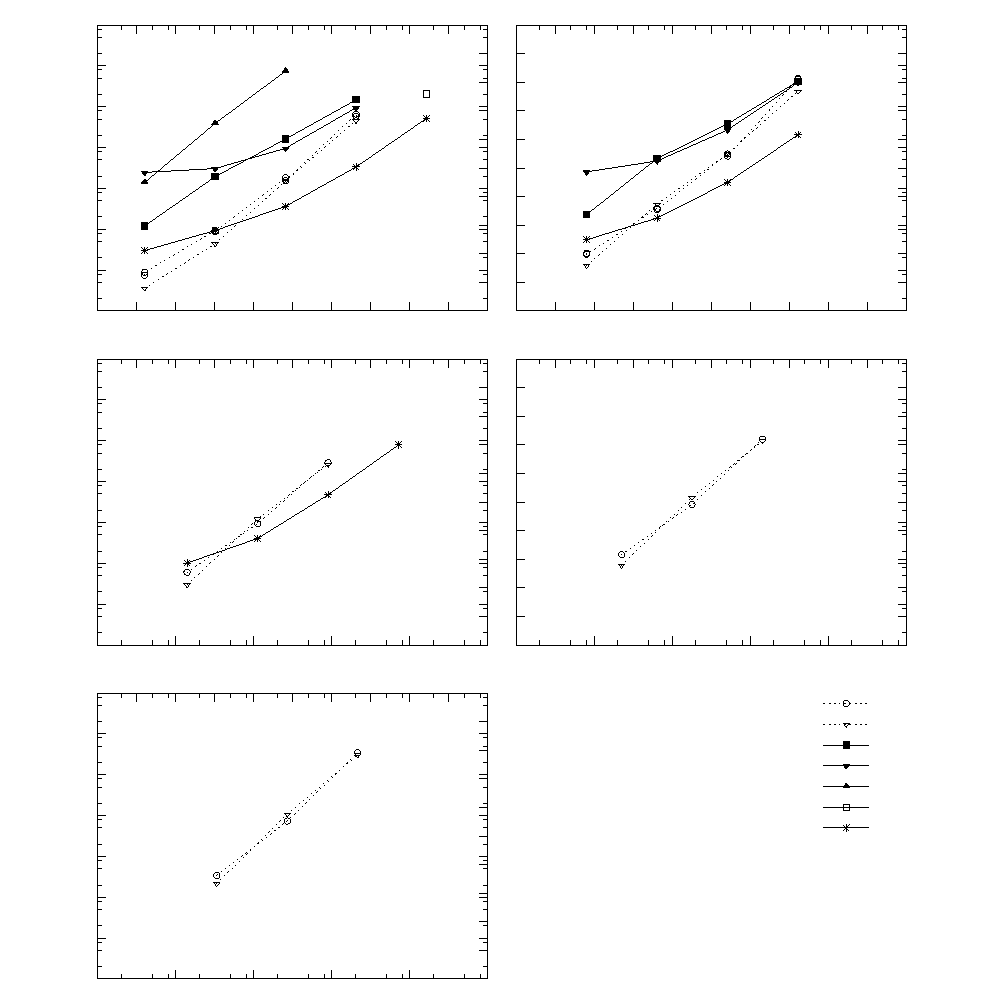
\includegraphics{ConstCoeffPoissonScaling}}%
    \gplfronttext
  \end{picture}%
\endgroup

	\end{center}
	\caption{
		Solver wallclock-time vs. degrees-of-freedom, for different polynomial degrees $k$,
		for problem/Equation (\ref{eq:ContantCoeffPoissonBenchmark}).
	}
	\label{fig:ConstantCoeffRuntimes}
\end{figure}

\newpage

\subsubsection{DG-Poisson: krylov-cycle Profiling}


\begin{figure}[!h]
	\begin{center}
		% GNUPLOT: LaTeX picture with Postscript
\begingroup
  \makeatletter
  \providecommand\color[2][]{%
    \GenericError{(gnuplot) \space\space\space\@spaces}{%
      Package color not loaded in conjunction with
      terminal option `colourtext'%
    }{See the gnuplot documentation for explanation.%
    }{Either use 'blacktext' in gnuplot or load the package
      color.sty in LaTeX.}%
    \renewcommand\color[2][]{}%
  }%
  \providecommand\includegraphics[2][]{%
    \GenericError{(gnuplot) \space\space\space\@spaces}{%
      Package graphicx or graphics not loaded%
    }{See the gnuplot documentation for explanation.%
    }{The gnuplot epslatex terminal needs graphicx.sty or graphics.sty.}%
    \renewcommand\includegraphics[2][]{}%
  }%
  \providecommand\rotatebox[2]{#2}%
  \@ifundefined{ifGPcolor}{%
    \newif\ifGPcolor
    \GPcolortrue
  }{}%
  \@ifundefined{ifGPblacktext}{%
    \newif\ifGPblacktext
    \GPblacktexttrue
  }{}%
  % define a \g@addto@macro without @ in the name:
  \let\gplgaddtomacro\g@addto@macro
  % define empty templates for all commands taking text:
  \gdef\gplbacktext{}%
  \gdef\gplfronttext{}%
  \makeatother
  \ifGPblacktext
    % no textcolor at all
    \def\colorrgb#1{}%
    \def\colorgray#1{}%
  \else
    % gray or color?
    \ifGPcolor
      \def\colorrgb#1{\color[rgb]{#1}}%
      \def\colorgray#1{\color[gray]{#1}}%
      \expandafter\def\csname LTw\endcsname{\color{white}}%
      \expandafter\def\csname LTb\endcsname{\color{black}}%
      \expandafter\def\csname LTa\endcsname{\color{black}}%
      \expandafter\def\csname LT0\endcsname{\color[rgb]{1,0,0}}%
      \expandafter\def\csname LT1\endcsname{\color[rgb]{0,1,0}}%
      \expandafter\def\csname LT2\endcsname{\color[rgb]{0,0,1}}%
      \expandafter\def\csname LT3\endcsname{\color[rgb]{1,0,1}}%
      \expandafter\def\csname LT4\endcsname{\color[rgb]{0,1,1}}%
      \expandafter\def\csname LT5\endcsname{\color[rgb]{1,1,0}}%
      \expandafter\def\csname LT6\endcsname{\color[rgb]{0,0,0}}%
      \expandafter\def\csname LT7\endcsname{\color[rgb]{1,0.3,0}}%
      \expandafter\def\csname LT8\endcsname{\color[rgb]{0.5,0.5,0.5}}%
    \else
      % gray
      \def\colorrgb#1{\color{black}}%
      \def\colorgray#1{\color[gray]{#1}}%
      \expandafter\def\csname LTw\endcsname{\color{white}}%
      \expandafter\def\csname LTb\endcsname{\color{black}}%
      \expandafter\def\csname LTa\endcsname{\color{black}}%
      \expandafter\def\csname LT0\endcsname{\color{black}}%
      \expandafter\def\csname LT1\endcsname{\color{black}}%
      \expandafter\def\csname LT2\endcsname{\color{black}}%
      \expandafter\def\csname LT3\endcsname{\color{black}}%
      \expandafter\def\csname LT4\endcsname{\color{black}}%
      \expandafter\def\csname LT5\endcsname{\color{black}}%
      \expandafter\def\csname LT6\endcsname{\color{black}}%
      \expandafter\def\csname LT7\endcsname{\color{black}}%
      \expandafter\def\csname LT8\endcsname{\color{black}}%
    \fi
  \fi
    \setlength{\unitlength}{0.0500bp}%
    \ifx\gptboxheight\undefined%
      \newlength{\gptboxheight}%
      \newlength{\gptboxwidth}%
      \newsavebox{\gptboxtext}%
    \fi%
    \setlength{\fboxrule}{0.5pt}%
    \setlength{\fboxsep}{1pt}%
\begin{picture}(7920.00,6800.00)%
    \gplgaddtomacro\gplbacktext{%
      \csname LTb\endcsname%
      \put(997,4735){\makebox(0,0)[r]{\strut{}$10^{-2}$}}%
      \csname LTb\endcsname%
      \put(997,5075){\makebox(0,0)[r]{\strut{}$10^{-1}$}}%
      \csname LTb\endcsname%
      \put(997,5415){\makebox(0,0)[r]{\strut{}$10^{0}$}}%
      \csname LTb\endcsname%
      \put(997,5755){\makebox(0,0)[r]{\strut{}$10^{1}$}}%
      \csname LTb\endcsname%
      \put(997,6096){\makebox(0,0)[r]{\strut{}$10^{2}$}}%
      \csname LTb\endcsname%
      \put(997,6436){\makebox(0,0)[r]{\strut{}$10^{3}$}}%
      \csname LTb\endcsname%
      \put(997,6776){\makebox(0,0)[r]{\strut{}$10^{4}$}}%
      \csname LTb\endcsname%
      \put(1099,4556){\makebox(0,0){\strut{} }}%
      \csname LTb\endcsname%
      \put(2137,4556){\makebox(0,0){\strut{} }}%
      \csname LTb\endcsname%
      \put(3176,4556){\makebox(0,0){\strut{} }}%
      \csname LTb\endcsname%
      \put(4214,4556){\makebox(0,0){\strut{} }}%
      \csname LTb\endcsname%
      \put(5252,4556){\makebox(0,0){\strut{} }}%
      \csname LTb\endcsname%
      \put(6291,4556){\makebox(0,0){\strut{} }}%
      \csname LTb\endcsname%
      \put(7329,4556){\makebox(0,0){\strut{} }}%
      \csname LTb\endcsname%
      \put(7431,4735){\makebox(0,0)[l]{\strut{} }}%
      \csname LTb\endcsname%
      \put(7431,5075){\makebox(0,0)[l]{\strut{} }}%
      \csname LTb\endcsname%
      \put(7431,5415){\makebox(0,0)[l]{\strut{} }}%
      \csname LTb\endcsname%
      \put(7431,5756){\makebox(0,0)[l]{\strut{} }}%
      \csname LTb\endcsname%
      \put(7431,6096){\makebox(0,0)[l]{\strut{} }}%
      \csname LTb\endcsname%
      \put(7431,6436){\makebox(0,0)[l]{\strut{} }}%
      \csname LTb\endcsname%
      \put(7431,6776){\makebox(0,0)[l]{\strut{} }}%
    }%
    \gplgaddtomacro\gplfronttext{%
      \csname LTb\endcsname%
      \put(397,5755){\rotatebox{-270}{\makebox(0,0){\strut{}$k = 2$}}}%
      \csname LTb\endcsname%
      \put(2190,6565){\makebox(0,0)[l]{\strut{}Slv Iter}}%
      \csname LTb\endcsname%
      \put(2190,6286){\makebox(0,0)[l]{\strut{}Slv Init}}%
      \csname LTb\endcsname%
      \put(2190,6007){\makebox(0,0)[l]{\strut{}Agg Init}}%
      \csname LTb\endcsname%
      \put(2190,5728){\makebox(0,0)[l]{\strut{}Mtx ass}}%
      \csname LTb\endcsname%
      \put(2190,5449){\makebox(0,0)[l]{\strut{}linear}}%
    }%
    \gplgaddtomacro\gplbacktext{%
      \csname LTb\endcsname%
      \put(997,2468){\makebox(0,0)[r]{\strut{}$10^{-2}$}}%
      \csname LTb\endcsname%
      \put(997,2808){\makebox(0,0)[r]{\strut{}$10^{-1}$}}%
      \csname LTb\endcsname%
      \put(997,3149){\makebox(0,0)[r]{\strut{}$10^{0}$}}%
      \csname LTb\endcsname%
      \put(997,3489){\makebox(0,0)[r]{\strut{}$10^{1}$}}%
      \csname LTb\endcsname%
      \put(997,3829){\makebox(0,0)[r]{\strut{}$10^{2}$}}%
      \csname LTb\endcsname%
      \put(997,4170){\makebox(0,0)[r]{\strut{}$10^{3}$}}%
      \csname LTb\endcsname%
      \put(997,4510){\makebox(0,0)[r]{\strut{}$10^{4}$}}%
      \csname LTb\endcsname%
      \put(1099,2289){\makebox(0,0){\strut{} }}%
      \csname LTb\endcsname%
      \put(2137,2289){\makebox(0,0){\strut{} }}%
      \csname LTb\endcsname%
      \put(3176,2289){\makebox(0,0){\strut{} }}%
      \csname LTb\endcsname%
      \put(4214,2289){\makebox(0,0){\strut{} }}%
      \csname LTb\endcsname%
      \put(5252,2289){\makebox(0,0){\strut{} }}%
      \csname LTb\endcsname%
      \put(6291,2289){\makebox(0,0){\strut{} }}%
      \csname LTb\endcsname%
      \put(7329,2289){\makebox(0,0){\strut{} }}%
      \csname LTb\endcsname%
      \put(7431,2468){\makebox(0,0)[l]{\strut{} }}%
      \csname LTb\endcsname%
      \put(7431,2808){\makebox(0,0)[l]{\strut{} }}%
      \csname LTb\endcsname%
      \put(7431,3149){\makebox(0,0)[l]{\strut{} }}%
      \csname LTb\endcsname%
      \put(7431,3489){\makebox(0,0)[l]{\strut{} }}%
      \csname LTb\endcsname%
      \put(7431,3829){\makebox(0,0)[l]{\strut{} }}%
      \csname LTb\endcsname%
      \put(7431,4170){\makebox(0,0)[l]{\strut{} }}%
      \csname LTb\endcsname%
      \put(7431,4510){\makebox(0,0)[l]{\strut{} }}%
      \csname LTb\endcsname%
      \put(1099,4689){\makebox(0,0){\strut{} }}%
      \csname LTb\endcsname%
      \put(2137,4689){\makebox(0,0){\strut{} }}%
      \csname LTb\endcsname%
      \put(3176,4689){\makebox(0,0){\strut{} }}%
      \csname LTb\endcsname%
      \put(4214,4689){\makebox(0,0){\strut{} }}%
      \csname LTb\endcsname%
      \put(5252,4689){\makebox(0,0){\strut{} }}%
      \csname LTb\endcsname%
      \put(6291,4689){\makebox(0,0){\strut{} }}%
      \csname LTb\endcsname%
      \put(7329,4689){\makebox(0,0){\strut{} }}%
    }%
    \gplgaddtomacro\gplfronttext{%
      \csname LTb\endcsname%
      \put(397,3489){\rotatebox{-270}{\makebox(0,0){\strut{}$k = 3$}}}%
    }%
    \gplgaddtomacro\gplbacktext{%
      \csname LTb\endcsname%
      \put(997,201){\makebox(0,0)[r]{\strut{}$10^{-2}$}}%
      \csname LTb\endcsname%
      \put(997,541){\makebox(0,0)[r]{\strut{}$10^{-1}$}}%
      \csname LTb\endcsname%
      \put(997,882){\makebox(0,0)[r]{\strut{}$10^{0}$}}%
      \csname LTb\endcsname%
      \put(997,1222){\makebox(0,0)[r]{\strut{}$10^{1}$}}%
      \csname LTb\endcsname%
      \put(997,1563){\makebox(0,0)[r]{\strut{}$10^{2}$}}%
      \csname LTb\endcsname%
      \put(997,1903){\makebox(0,0)[r]{\strut{}$10^{3}$}}%
      \csname LTb\endcsname%
      \put(997,2244){\makebox(0,0)[r]{\strut{}$10^{4}$}}%
      \csname LTb\endcsname%
      \put(7431,201){\makebox(0,0)[l]{\strut{} }}%
      \csname LTb\endcsname%
      \put(7431,542){\makebox(0,0)[l]{\strut{} }}%
      \csname LTb\endcsname%
      \put(7431,882){\makebox(0,0)[l]{\strut{} }}%
      \csname LTb\endcsname%
      \put(7431,1223){\makebox(0,0)[l]{\strut{} }}%
      \csname LTb\endcsname%
      \put(7431,1563){\makebox(0,0)[l]{\strut{} }}%
      \csname LTb\endcsname%
      \put(7431,1904){\makebox(0,0)[l]{\strut{} }}%
      \csname LTb\endcsname%
      \put(7431,2244){\makebox(0,0)[l]{\strut{} }}%
      \csname LTb\endcsname%
      \put(1099,2423){\makebox(0,0){\strut{} }}%
      \csname LTb\endcsname%
      \put(2137,2423){\makebox(0,0){\strut{} }}%
      \csname LTb\endcsname%
      \put(3176,2423){\makebox(0,0){\strut{} }}%
      \csname LTb\endcsname%
      \put(4214,2423){\makebox(0,0){\strut{} }}%
      \csname LTb\endcsname%
      \put(5252,2423){\makebox(0,0){\strut{} }}%
      \csname LTb\endcsname%
      \put(6291,2423){\makebox(0,0){\strut{} }}%
      \csname LTb\endcsname%
      \put(7329,2423){\makebox(0,0){\strut{} }}%
    }%
    \gplgaddtomacro\gplfronttext{%
      \csname LTb\endcsname%
      \put(397,1222){\rotatebox{-270}{\makebox(0,0){\strut{}$k = 5$}}}%
    }%
    \gplbacktext
    \put(0,0){\includegraphics{ConstCoeffPoissonexp_Kcycle_schwarz}}%
    \gplfronttext
  \end{picture}%
\endgroup

	\end{center}
	\caption{
		Investigation of runtime of different code parts of the V-kcycle with additive Schwarz (p-two-grid as block solver) smoother. wallclock-time vs. degrees-of-freedom, for different polynomial degrees $k$,
		for problem/Equation (\ref{eq:ContantCoeffPoissonBenchmark}).
	}
	\label{fig:SIP_blockJacobianPCG}
\end{figure}
\newpage

\subsubsection{DG-Poisson: preconditioned GMRES Profiling}

\begin{figure}[!h]
	\begin{center}
		% GNUPLOT: LaTeX picture with Postscript
\begingroup
  \makeatletter
  \providecommand\color[2][]{%
    \GenericError{(gnuplot) \space\space\space\@spaces}{%
      Package color not loaded in conjunction with
      terminal option `colourtext'%
    }{See the gnuplot documentation for explanation.%
    }{Either use 'blacktext' in gnuplot or load the package
      color.sty in LaTeX.}%
    \renewcommand\color[2][]{}%
  }%
  \providecommand\includegraphics[2][]{%
    \GenericError{(gnuplot) \space\space\space\@spaces}{%
      Package graphicx or graphics not loaded%
    }{See the gnuplot documentation for explanation.%
    }{The gnuplot epslatex terminal needs graphicx.sty or graphics.sty.}%
    \renewcommand\includegraphics[2][]{}%
  }%
  \providecommand\rotatebox[2]{#2}%
  \@ifundefined{ifGPcolor}{%
    \newif\ifGPcolor
    \GPcolortrue
  }{}%
  \@ifundefined{ifGPblacktext}{%
    \newif\ifGPblacktext
    \GPblacktexttrue
  }{}%
  % define a \g@addto@macro without @ in the name:
  \let\gplgaddtomacro\g@addto@macro
  % define empty templates for all commands taking text:
  \gdef\gplbacktext{}%
  \gdef\gplfronttext{}%
  \makeatother
  \ifGPblacktext
    % no textcolor at all
    \def\colorrgb#1{}%
    \def\colorgray#1{}%
  \else
    % gray or color?
    \ifGPcolor
      \def\colorrgb#1{\color[rgb]{#1}}%
      \def\colorgray#1{\color[gray]{#1}}%
      \expandafter\def\csname LTw\endcsname{\color{white}}%
      \expandafter\def\csname LTb\endcsname{\color{black}}%
      \expandafter\def\csname LTa\endcsname{\color{black}}%
      \expandafter\def\csname LT0\endcsname{\color[rgb]{1,0,0}}%
      \expandafter\def\csname LT1\endcsname{\color[rgb]{0,1,0}}%
      \expandafter\def\csname LT2\endcsname{\color[rgb]{0,0,1}}%
      \expandafter\def\csname LT3\endcsname{\color[rgb]{1,0,1}}%
      \expandafter\def\csname LT4\endcsname{\color[rgb]{0,1,1}}%
      \expandafter\def\csname LT5\endcsname{\color[rgb]{1,1,0}}%
      \expandafter\def\csname LT6\endcsname{\color[rgb]{0,0,0}}%
      \expandafter\def\csname LT7\endcsname{\color[rgb]{1,0.3,0}}%
      \expandafter\def\csname LT8\endcsname{\color[rgb]{0.5,0.5,0.5}}%
    \else
      % gray
      \def\colorrgb#1{\color{black}}%
      \def\colorgray#1{\color[gray]{#1}}%
      \expandafter\def\csname LTw\endcsname{\color{white}}%
      \expandafter\def\csname LTb\endcsname{\color{black}}%
      \expandafter\def\csname LTa\endcsname{\color{black}}%
      \expandafter\def\csname LT0\endcsname{\color{black}}%
      \expandafter\def\csname LT1\endcsname{\color{black}}%
      \expandafter\def\csname LT2\endcsname{\color{black}}%
      \expandafter\def\csname LT3\endcsname{\color{black}}%
      \expandafter\def\csname LT4\endcsname{\color{black}}%
      \expandafter\def\csname LT5\endcsname{\color{black}}%
      \expandafter\def\csname LT6\endcsname{\color{black}}%
      \expandafter\def\csname LT7\endcsname{\color{black}}%
      \expandafter\def\csname LT8\endcsname{\color{black}}%
    \fi
  \fi
    \setlength{\unitlength}{0.0500bp}%
    \ifx\gptboxheight\undefined%
      \newlength{\gptboxheight}%
      \newlength{\gptboxwidth}%
      \newsavebox{\gptboxtext}%
    \fi%
    \setlength{\fboxrule}{0.5pt}%
    \setlength{\fboxsep}{1pt}%
\begin{picture}(7920.00,6800.00)%
    \gplgaddtomacro\gplbacktext{%
      \csname LTb\endcsname%
      \put(997,4735){\makebox(0,0)[r]{\strut{}$10^{-2}$}}%
      \csname LTb\endcsname%
      \put(997,5075){\makebox(0,0)[r]{\strut{}$10^{-1}$}}%
      \csname LTb\endcsname%
      \put(997,5415){\makebox(0,0)[r]{\strut{}$10^{0}$}}%
      \csname LTb\endcsname%
      \put(997,5755){\makebox(0,0)[r]{\strut{}$10^{1}$}}%
      \csname LTb\endcsname%
      \put(997,6096){\makebox(0,0)[r]{\strut{}$10^{2}$}}%
      \csname LTb\endcsname%
      \put(997,6436){\makebox(0,0)[r]{\strut{}$10^{3}$}}%
      \csname LTb\endcsname%
      \put(997,6776){\makebox(0,0)[r]{\strut{}$10^{4}$}}%
      \csname LTb\endcsname%
      \put(1099,4556){\makebox(0,0){\strut{} }}%
      \csname LTb\endcsname%
      \put(2137,4556){\makebox(0,0){\strut{} }}%
      \csname LTb\endcsname%
      \put(3176,4556){\makebox(0,0){\strut{} }}%
      \csname LTb\endcsname%
      \put(4214,4556){\makebox(0,0){\strut{} }}%
      \csname LTb\endcsname%
      \put(5252,4556){\makebox(0,0){\strut{} }}%
      \csname LTb\endcsname%
      \put(6291,4556){\makebox(0,0){\strut{} }}%
      \csname LTb\endcsname%
      \put(7329,4556){\makebox(0,0){\strut{} }}%
      \csname LTb\endcsname%
      \put(7431,4735){\makebox(0,0)[l]{\strut{} }}%
      \csname LTb\endcsname%
      \put(7431,5075){\makebox(0,0)[l]{\strut{} }}%
      \csname LTb\endcsname%
      \put(7431,5415){\makebox(0,0)[l]{\strut{} }}%
      \csname LTb\endcsname%
      \put(7431,5756){\makebox(0,0)[l]{\strut{} }}%
      \csname LTb\endcsname%
      \put(7431,6096){\makebox(0,0)[l]{\strut{} }}%
      \csname LTb\endcsname%
      \put(7431,6436){\makebox(0,0)[l]{\strut{} }}%
      \csname LTb\endcsname%
      \put(7431,6776){\makebox(0,0)[l]{\strut{} }}%
    }%
    \gplgaddtomacro\gplfronttext{%
      \csname LTb\endcsname%
      \put(397,5755){\rotatebox{-270}{\makebox(0,0){\strut{}$k = 2$}}}%
      \csname LTb\endcsname%
      \put(2190,6565){\makebox(0,0)[l]{\strut{}Slv Iter}}%
      \csname LTb\endcsname%
      \put(2190,6286){\makebox(0,0)[l]{\strut{}Slv Init}}%
      \csname LTb\endcsname%
      \put(2190,6007){\makebox(0,0)[l]{\strut{}Agg Init}}%
      \csname LTb\endcsname%
      \put(2190,5728){\makebox(0,0)[l]{\strut{}Mtx ass}}%
      \csname LTb\endcsname%
      \put(2190,5449){\makebox(0,0)[l]{\strut{}linear}}%
    }%
    \gplgaddtomacro\gplbacktext{%
      \csname LTb\endcsname%
      \put(997,2468){\makebox(0,0)[r]{\strut{}$10^{-2}$}}%
      \csname LTb\endcsname%
      \put(997,2808){\makebox(0,0)[r]{\strut{}$10^{-1}$}}%
      \csname LTb\endcsname%
      \put(997,3149){\makebox(0,0)[r]{\strut{}$10^{0}$}}%
      \csname LTb\endcsname%
      \put(997,3489){\makebox(0,0)[r]{\strut{}$10^{1}$}}%
      \csname LTb\endcsname%
      \put(997,3829){\makebox(0,0)[r]{\strut{}$10^{2}$}}%
      \csname LTb\endcsname%
      \put(997,4170){\makebox(0,0)[r]{\strut{}$10^{3}$}}%
      \csname LTb\endcsname%
      \put(997,4510){\makebox(0,0)[r]{\strut{}$10^{4}$}}%
      \csname LTb\endcsname%
      \put(1099,2289){\makebox(0,0){\strut{} }}%
      \csname LTb\endcsname%
      \put(2137,2289){\makebox(0,0){\strut{} }}%
      \csname LTb\endcsname%
      \put(3176,2289){\makebox(0,0){\strut{} }}%
      \csname LTb\endcsname%
      \put(4214,2289){\makebox(0,0){\strut{} }}%
      \csname LTb\endcsname%
      \put(5252,2289){\makebox(0,0){\strut{} }}%
      \csname LTb\endcsname%
      \put(6291,2289){\makebox(0,0){\strut{} }}%
      \csname LTb\endcsname%
      \put(7329,2289){\makebox(0,0){\strut{} }}%
      \csname LTb\endcsname%
      \put(7431,2468){\makebox(0,0)[l]{\strut{} }}%
      \csname LTb\endcsname%
      \put(7431,2808){\makebox(0,0)[l]{\strut{} }}%
      \csname LTb\endcsname%
      \put(7431,3149){\makebox(0,0)[l]{\strut{} }}%
      \csname LTb\endcsname%
      \put(7431,3489){\makebox(0,0)[l]{\strut{} }}%
      \csname LTb\endcsname%
      \put(7431,3829){\makebox(0,0)[l]{\strut{} }}%
      \csname LTb\endcsname%
      \put(7431,4170){\makebox(0,0)[l]{\strut{} }}%
      \csname LTb\endcsname%
      \put(7431,4510){\makebox(0,0)[l]{\strut{} }}%
      \csname LTb\endcsname%
      \put(1099,4689){\makebox(0,0){\strut{} }}%
      \csname LTb\endcsname%
      \put(2137,4689){\makebox(0,0){\strut{} }}%
      \csname LTb\endcsname%
      \put(3176,4689){\makebox(0,0){\strut{} }}%
      \csname LTb\endcsname%
      \put(4214,4689){\makebox(0,0){\strut{} }}%
      \csname LTb\endcsname%
      \put(5252,4689){\makebox(0,0){\strut{} }}%
      \csname LTb\endcsname%
      \put(6291,4689){\makebox(0,0){\strut{} }}%
      \csname LTb\endcsname%
      \put(7329,4689){\makebox(0,0){\strut{} }}%
    }%
    \gplgaddtomacro\gplfronttext{%
      \csname LTb\endcsname%
      \put(397,3489){\rotatebox{-270}{\makebox(0,0){\strut{}$k = 3$}}}%
    }%
    \gplgaddtomacro\gplbacktext{%
      \csname LTb\endcsname%
      \put(997,201){\makebox(0,0)[r]{\strut{}$10^{-2}$}}%
      \csname LTb\endcsname%
      \put(997,541){\makebox(0,0)[r]{\strut{}$10^{-1}$}}%
      \csname LTb\endcsname%
      \put(997,882){\makebox(0,0)[r]{\strut{}$10^{0}$}}%
      \csname LTb\endcsname%
      \put(997,1222){\makebox(0,0)[r]{\strut{}$10^{1}$}}%
      \csname LTb\endcsname%
      \put(997,1563){\makebox(0,0)[r]{\strut{}$10^{2}$}}%
      \csname LTb\endcsname%
      \put(997,1903){\makebox(0,0)[r]{\strut{}$10^{3}$}}%
      \csname LTb\endcsname%
      \put(997,2244){\makebox(0,0)[r]{\strut{}$10^{4}$}}%
      \csname LTb\endcsname%
      \put(7431,201){\makebox(0,0)[l]{\strut{} }}%
      \csname LTb\endcsname%
      \put(7431,542){\makebox(0,0)[l]{\strut{} }}%
      \csname LTb\endcsname%
      \put(7431,882){\makebox(0,0)[l]{\strut{} }}%
      \csname LTb\endcsname%
      \put(7431,1223){\makebox(0,0)[l]{\strut{} }}%
      \csname LTb\endcsname%
      \put(7431,1563){\makebox(0,0)[l]{\strut{} }}%
      \csname LTb\endcsname%
      \put(7431,1904){\makebox(0,0)[l]{\strut{} }}%
      \csname LTb\endcsname%
      \put(7431,2244){\makebox(0,0)[l]{\strut{} }}%
      \csname LTb\endcsname%
      \put(1099,2423){\makebox(0,0){\strut{} }}%
      \csname LTb\endcsname%
      \put(2137,2423){\makebox(0,0){\strut{} }}%
      \csname LTb\endcsname%
      \put(3176,2423){\makebox(0,0){\strut{} }}%
      \csname LTb\endcsname%
      \put(4214,2423){\makebox(0,0){\strut{} }}%
      \csname LTb\endcsname%
      \put(5252,2423){\makebox(0,0){\strut{} }}%
      \csname LTb\endcsname%
      \put(6291,2423){\makebox(0,0){\strut{} }}%
      \csname LTb\endcsname%
      \put(7329,2423){\makebox(0,0){\strut{} }}%
    }%
    \gplgaddtomacro\gplfronttext{%
      \csname LTb\endcsname%
      \put(397,1222){\rotatebox{-270}{\makebox(0,0){\strut{}$k = 5$}}}%
    }%
    \gplbacktext
    \put(0,0){\includegraphics{ConstCoeffPoissonexp_gmres_levelpmg}}%
    \gplfronttext
  \end{picture}%
\endgroup

	\end{center}
	\caption{
		Investigation of runtime of different code parts of the preconditioned GMRES algorithm. Wallclock-time vs. degrees-of-freedom, for different polynomial degrees $k$,
		for problem/Equation (\ref{eq:ContantCoeffPoissonBenchmark}).
	}
	\label{fig:SIP_SchwarzPGC}
\end{figure}
\newpage

\subsection{Xdg-Poisson test problem}
\label{sec:XdgPoisson}

\newcommand{\frakA}{\mathfrak{A}}
\newcommand{\frakB}{\mathfrak{B}}
\newcommand{\nOmega}{\vec{n}_{\partial \Omega } }
%\newcommand*{\jump}[1]{\left\llbracket {#1} \right\rrbracket}
\newcommand{\frakI}{\mathfrak{I}}
\newcommand{\nI}{\vec{n}_\frakI}

The test problem can be considered as stationary 3 dimensional heat equation with source-term and with two phases:
\begin{equation}
\left\{ \begin{array}{rll}
- \mu \Delta u                   & = f               & \text{ in } \Omega \setminus \frakI , \\
\jump{u}                         & = 0               & \text{ on } \frakI ,                  \\
\jump{\mu \nabla u \cdot \nI}    & = 0               & \text{ on } \frakI ,                  \\
u                                & = g_\text{Diri}   & \text{ on } \Gamma_\mathrm{Diri} ,    \\
\nabla u \cdot \nOmega           & = g_\text{Neu}    & \text{ on } \Gamma_\mathrm{Neu} .     \\
\end{array}
\right.
\label{eq:XdgPoissonBenchmark}
\end{equation}
with a constant diffusion coefficient in each subdomain


\begin{equation}
\mu (\vec{x}) = 
\left\{ \begin{array}{ll}
\mu_\frakA & \text{for } \vec{x} \in \frakA, \\
\mu_\frakB & \text{for } \vec{x} \in \frakB. \\
\end{array} \right.
\label{eq:DiscDiffKoeff}
\end{equation}

where $\mu_1=1$ (inner) and $\mu_2=1000$ (outer) characterize the two phases. is investigated on a uniform, equidistant Cartesian grid. See \ref{fig:XdgRuntimes} for results.

\graphicspath{{./apdx-NodeSolverPerformance/XDGPoisson/plots/}}

\subsubsection{Xdg-Poisson: scaling of solvers}

\begin{figure}[!h]
	\begin{center}
		% GNUPLOT: LaTeX picture with Postscript
\begingroup
  \makeatletter
  \providecommand\color[2][]{%
    \GenericError{(gnuplot) \space\space\space\@spaces}{%
      Package color not loaded in conjunction with
      terminal option `colourtext'%
    }{See the gnuplot documentation for explanation.%
    }{Either use 'blacktext' in gnuplot or load the package
      color.sty in LaTeX.}%
    \renewcommand\color[2][]{}%
  }%
  \providecommand\includegraphics[2][]{%
    \GenericError{(gnuplot) \space\space\space\@spaces}{%
      Package graphicx or graphics not loaded%
    }{See the gnuplot documentation for explanation.%
    }{The gnuplot epslatex terminal needs graphicx.sty or graphics.sty.}%
    \renewcommand\includegraphics[2][]{}%
  }%
  \providecommand\rotatebox[2]{#2}%
  \@ifundefined{ifGPcolor}{%
    \newif\ifGPcolor
    \GPcolortrue
  }{}%
  \@ifundefined{ifGPblacktext}{%
    \newif\ifGPblacktext
    \GPblacktexttrue
  }{}%
  % define a \g@addto@macro without @ in the name:
  \let\gplgaddtomacro\g@addto@macro
  % define empty templates for all commands taking text:
  \gdef\gplbacktext{}%
  \gdef\gplfronttext{}%
  \makeatother
  \ifGPblacktext
    % no textcolor at all
    \def\colorrgb#1{}%
    \def\colorgray#1{}%
  \else
    % gray or color?
    \ifGPcolor
      \def\colorrgb#1{\color[rgb]{#1}}%
      \def\colorgray#1{\color[gray]{#1}}%
      \expandafter\def\csname LTw\endcsname{\color{white}}%
      \expandafter\def\csname LTb\endcsname{\color{black}}%
      \expandafter\def\csname LTa\endcsname{\color{black}}%
      \expandafter\def\csname LT0\endcsname{\color[rgb]{1,0,0}}%
      \expandafter\def\csname LT1\endcsname{\color[rgb]{0,1,0}}%
      \expandafter\def\csname LT2\endcsname{\color[rgb]{0,0,1}}%
      \expandafter\def\csname LT3\endcsname{\color[rgb]{1,0,1}}%
      \expandafter\def\csname LT4\endcsname{\color[rgb]{0,1,1}}%
      \expandafter\def\csname LT5\endcsname{\color[rgb]{1,1,0}}%
      \expandafter\def\csname LT6\endcsname{\color[rgb]{0,0,0}}%
      \expandafter\def\csname LT7\endcsname{\color[rgb]{1,0.3,0}}%
      \expandafter\def\csname LT8\endcsname{\color[rgb]{0.5,0.5,0.5}}%
    \else
      % gray
      \def\colorrgb#1{\color{black}}%
      \def\colorgray#1{\color[gray]{#1}}%
      \expandafter\def\csname LTw\endcsname{\color{white}}%
      \expandafter\def\csname LTb\endcsname{\color{black}}%
      \expandafter\def\csname LTa\endcsname{\color{black}}%
      \expandafter\def\csname LT0\endcsname{\color{black}}%
      \expandafter\def\csname LT1\endcsname{\color{black}}%
      \expandafter\def\csname LT2\endcsname{\color{black}}%
      \expandafter\def\csname LT3\endcsname{\color{black}}%
      \expandafter\def\csname LT4\endcsname{\color{black}}%
      \expandafter\def\csname LT5\endcsname{\color{black}}%
      \expandafter\def\csname LT6\endcsname{\color{black}}%
      \expandafter\def\csname LT7\endcsname{\color{black}}%
      \expandafter\def\csname LT8\endcsname{\color{black}}%
    \fi
  \fi
    \setlength{\unitlength}{0.0500bp}%
    \ifx\gptboxheight\undefined%
      \newlength{\gptboxheight}%
      \newlength{\gptboxwidth}%
      \newsavebox{\gptboxtext}%
    \fi%
    \setlength{\fboxrule}{0.5pt}%
    \setlength{\fboxsep}{1pt}%
\begin{picture}(7920.00,6800.00)%
    \gplgaddtomacro\gplbacktext{%
      \csname LTb\endcsname%
      \put(997,4735){\makebox(0,0)[r]{\strut{}$10^{-1}$}}%
      \csname LTb\endcsname%
      \put(997,5075){\makebox(0,0)[r]{\strut{}$10^{0}$}}%
      \csname LTb\endcsname%
      \put(997,5415){\makebox(0,0)[r]{\strut{}$10^{1}$}}%
      \csname LTb\endcsname%
      \put(997,5755){\makebox(0,0)[r]{\strut{}$10^{2}$}}%
      \csname LTb\endcsname%
      \put(997,6096){\makebox(0,0)[r]{\strut{}$10^{3}$}}%
      \csname LTb\endcsname%
      \put(997,6436){\makebox(0,0)[r]{\strut{}$10^{4}$}}%
      \csname LTb\endcsname%
      \put(997,6776){\makebox(0,0)[r]{\strut{}$10^{5}$}}%
      \csname LTb\endcsname%
      \put(1099,4556){\makebox(0,0){\strut{} }}%
      \csname LTb\endcsname%
      \put(2137,4556){\makebox(0,0){\strut{} }}%
      \csname LTb\endcsname%
      \put(3176,4556){\makebox(0,0){\strut{} }}%
      \csname LTb\endcsname%
      \put(4214,4556){\makebox(0,0){\strut{} }}%
      \csname LTb\endcsname%
      \put(5252,4556){\makebox(0,0){\strut{} }}%
      \csname LTb\endcsname%
      \put(6291,4556){\makebox(0,0){\strut{} }}%
      \csname LTb\endcsname%
      \put(7329,4556){\makebox(0,0){\strut{} }}%
      \csname LTb\endcsname%
      \put(7431,4735){\makebox(0,0)[l]{\strut{} }}%
      \csname LTb\endcsname%
      \put(7431,5075){\makebox(0,0)[l]{\strut{} }}%
      \csname LTb\endcsname%
      \put(7431,5415){\makebox(0,0)[l]{\strut{} }}%
      \csname LTb\endcsname%
      \put(7431,5756){\makebox(0,0)[l]{\strut{} }}%
      \csname LTb\endcsname%
      \put(7431,6096){\makebox(0,0)[l]{\strut{} }}%
      \csname LTb\endcsname%
      \put(7431,6436){\makebox(0,0)[l]{\strut{} }}%
      \csname LTb\endcsname%
      \put(7431,6776){\makebox(0,0)[l]{\strut{} }}%
    }%
    \gplgaddtomacro\gplfronttext{%
      \csname LTb\endcsname%
      \put(397,5755){\rotatebox{-270}{\makebox(0,0){\strut{}$k = 2$}}}%
      \csname LTb\endcsname%
      \put(2190,6565){\makebox(0,0)[l]{\strut{}Pardiso}}%
      \csname LTb\endcsname%
      \put(2190,6286){\makebox(0,0)[l]{\strut{}GMRES w. pTG}}%
      \csname LTb\endcsname%
      \put(2190,6007){\makebox(0,0)[l]{\strut{}Kcycle w. add.-Schwarz}}%
      \csname LTb\endcsname%
      \put(2190,5728){\makebox(0,0)[l]{\strut{}linear}}%
    }%
    \gplgaddtomacro\gplbacktext{%
      \csname LTb\endcsname%
      \put(997,2468){\makebox(0,0)[r]{\strut{}$10^{-1}$}}%
      \csname LTb\endcsname%
      \put(997,2808){\makebox(0,0)[r]{\strut{}$10^{0}$}}%
      \csname LTb\endcsname%
      \put(997,3149){\makebox(0,0)[r]{\strut{}$10^{1}$}}%
      \csname LTb\endcsname%
      \put(997,3489){\makebox(0,0)[r]{\strut{}$10^{2}$}}%
      \csname LTb\endcsname%
      \put(997,3829){\makebox(0,0)[r]{\strut{}$10^{3}$}}%
      \csname LTb\endcsname%
      \put(997,4170){\makebox(0,0)[r]{\strut{}$10^{4}$}}%
      \csname LTb\endcsname%
      \put(997,4510){\makebox(0,0)[r]{\strut{}$10^{5}$}}%
      \csname LTb\endcsname%
      \put(1099,2289){\makebox(0,0){\strut{} }}%
      \csname LTb\endcsname%
      \put(2137,2289){\makebox(0,0){\strut{} }}%
      \csname LTb\endcsname%
      \put(3176,2289){\makebox(0,0){\strut{} }}%
      \csname LTb\endcsname%
      \put(4214,2289){\makebox(0,0){\strut{} }}%
      \csname LTb\endcsname%
      \put(5252,2289){\makebox(0,0){\strut{} }}%
      \csname LTb\endcsname%
      \put(6291,2289){\makebox(0,0){\strut{} }}%
      \csname LTb\endcsname%
      \put(7329,2289){\makebox(0,0){\strut{} }}%
      \csname LTb\endcsname%
      \put(7431,2468){\makebox(0,0)[l]{\strut{} }}%
      \csname LTb\endcsname%
      \put(7431,2808){\makebox(0,0)[l]{\strut{} }}%
      \csname LTb\endcsname%
      \put(7431,3149){\makebox(0,0)[l]{\strut{} }}%
      \csname LTb\endcsname%
      \put(7431,3489){\makebox(0,0)[l]{\strut{} }}%
      \csname LTb\endcsname%
      \put(7431,3829){\makebox(0,0)[l]{\strut{} }}%
      \csname LTb\endcsname%
      \put(7431,4170){\makebox(0,0)[l]{\strut{} }}%
      \csname LTb\endcsname%
      \put(7431,4510){\makebox(0,0)[l]{\strut{} }}%
      \csname LTb\endcsname%
      \put(1099,4689){\makebox(0,0){\strut{} }}%
      \csname LTb\endcsname%
      \put(2137,4689){\makebox(0,0){\strut{} }}%
      \csname LTb\endcsname%
      \put(3176,4689){\makebox(0,0){\strut{} }}%
      \csname LTb\endcsname%
      \put(4214,4689){\makebox(0,0){\strut{} }}%
      \csname LTb\endcsname%
      \put(5252,4689){\makebox(0,0){\strut{} }}%
      \csname LTb\endcsname%
      \put(6291,4689){\makebox(0,0){\strut{} }}%
      \csname LTb\endcsname%
      \put(7329,4689){\makebox(0,0){\strut{} }}%
    }%
    \gplgaddtomacro\gplfronttext{%
      \csname LTb\endcsname%
      \put(397,3489){\rotatebox{-270}{\makebox(0,0){\strut{}$k = 3$}}}%
    }%
    \gplgaddtomacro\gplbacktext{%
      \csname LTb\endcsname%
      \put(997,201){\makebox(0,0)[r]{\strut{}$10^{-1}$}}%
      \csname LTb\endcsname%
      \put(997,541){\makebox(0,0)[r]{\strut{}$10^{0}$}}%
      \csname LTb\endcsname%
      \put(997,882){\makebox(0,0)[r]{\strut{}$10^{1}$}}%
      \csname LTb\endcsname%
      \put(997,1222){\makebox(0,0)[r]{\strut{}$10^{2}$}}%
      \csname LTb\endcsname%
      \put(997,1563){\makebox(0,0)[r]{\strut{}$10^{3}$}}%
      \csname LTb\endcsname%
      \put(997,1903){\makebox(0,0)[r]{\strut{}$10^{4}$}}%
      \csname LTb\endcsname%
      \put(997,2244){\makebox(0,0)[r]{\strut{}$10^{5}$}}%
      \csname LTb\endcsname%
      \put(7431,201){\makebox(0,0)[l]{\strut{} }}%
      \csname LTb\endcsname%
      \put(7431,542){\makebox(0,0)[l]{\strut{} }}%
      \csname LTb\endcsname%
      \put(7431,882){\makebox(0,0)[l]{\strut{} }}%
      \csname LTb\endcsname%
      \put(7431,1223){\makebox(0,0)[l]{\strut{} }}%
      \csname LTb\endcsname%
      \put(7431,1563){\makebox(0,0)[l]{\strut{} }}%
      \csname LTb\endcsname%
      \put(7431,1904){\makebox(0,0)[l]{\strut{} }}%
      \csname LTb\endcsname%
      \put(7431,2244){\makebox(0,0)[l]{\strut{} }}%
      \csname LTb\endcsname%
      \put(1099,2423){\makebox(0,0){\strut{} }}%
      \csname LTb\endcsname%
      \put(2137,2423){\makebox(0,0){\strut{} }}%
      \csname LTb\endcsname%
      \put(3176,2423){\makebox(0,0){\strut{} }}%
      \csname LTb\endcsname%
      \put(4214,2423){\makebox(0,0){\strut{} }}%
      \csname LTb\endcsname%
      \put(5252,2423){\makebox(0,0){\strut{} }}%
      \csname LTb\endcsname%
      \put(6291,2423){\makebox(0,0){\strut{} }}%
      \csname LTb\endcsname%
      \put(7329,2423){\makebox(0,0){\strut{} }}%
    }%
    \gplgaddtomacro\gplfronttext{%
      \csname LTb\endcsname%
      \put(397,1222){\rotatebox{-270}{\makebox(0,0){\strut{}$k = 5$}}}%
    }%
    \gplbacktext
    \put(0,0){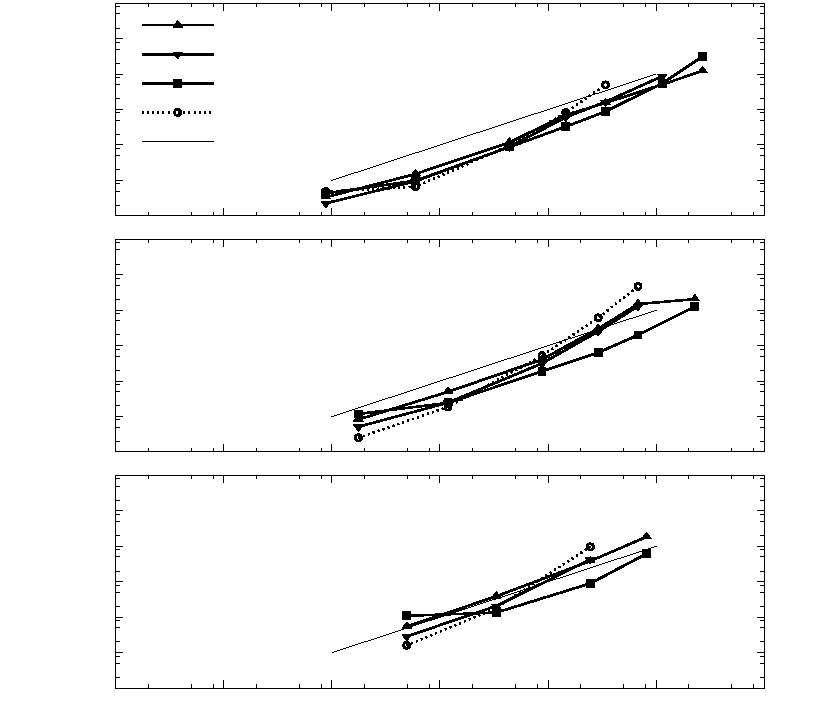
\includegraphics{XdgPoissonScaling}}%
    \gplfronttext
  \end{picture}%
\endgroup

	\end{center}
	\caption{
		Solver runtime vs. degrees-of-freedom, for different polynomial degrees $k$,
		for problem/Equation (\ref{eq:XdgPoissonBenchmark}).
	}
	\label{fig:XdgRuntimes}
\end{figure}
\newpage

\subsubsection{Xdg-Poisson: krylov-cycle Profiling}


\begin{figure}[!h]
	\begin{center}
		% GNUPLOT: LaTeX picture with Postscript
\begingroup
  \makeatletter
  \providecommand\color[2][]{%
    \GenericError{(gnuplot) \space\space\space\@spaces}{%
      Package color not loaded in conjunction with
      terminal option `colourtext'%
    }{See the gnuplot documentation for explanation.%
    }{Either use 'blacktext' in gnuplot or load the package
      color.sty in LaTeX.}%
    \renewcommand\color[2][]{}%
  }%
  \providecommand\includegraphics[2][]{%
    \GenericError{(gnuplot) \space\space\space\@spaces}{%
      Package graphicx or graphics not loaded%
    }{See the gnuplot documentation for explanation.%
    }{The gnuplot epslatex terminal needs graphicx.sty or graphics.sty.}%
    \renewcommand\includegraphics[2][]{}%
  }%
  \providecommand\rotatebox[2]{#2}%
  \@ifundefined{ifGPcolor}{%
    \newif\ifGPcolor
    \GPcolortrue
  }{}%
  \@ifundefined{ifGPblacktext}{%
    \newif\ifGPblacktext
    \GPblacktexttrue
  }{}%
  % define a \g@addto@macro without @ in the name:
  \let\gplgaddtomacro\g@addto@macro
  % define empty templates for all commands taking text:
  \gdef\gplbacktext{}%
  \gdef\gplfronttext{}%
  \makeatother
  \ifGPblacktext
    % no textcolor at all
    \def\colorrgb#1{}%
    \def\colorgray#1{}%
  \else
    % gray or color?
    \ifGPcolor
      \def\colorrgb#1{\color[rgb]{#1}}%
      \def\colorgray#1{\color[gray]{#1}}%
      \expandafter\def\csname LTw\endcsname{\color{white}}%
      \expandafter\def\csname LTb\endcsname{\color{black}}%
      \expandafter\def\csname LTa\endcsname{\color{black}}%
      \expandafter\def\csname LT0\endcsname{\color[rgb]{1,0,0}}%
      \expandafter\def\csname LT1\endcsname{\color[rgb]{0,1,0}}%
      \expandafter\def\csname LT2\endcsname{\color[rgb]{0,0,1}}%
      \expandafter\def\csname LT3\endcsname{\color[rgb]{1,0,1}}%
      \expandafter\def\csname LT4\endcsname{\color[rgb]{0,1,1}}%
      \expandafter\def\csname LT5\endcsname{\color[rgb]{1,1,0}}%
      \expandafter\def\csname LT6\endcsname{\color[rgb]{0,0,0}}%
      \expandafter\def\csname LT7\endcsname{\color[rgb]{1,0.3,0}}%
      \expandafter\def\csname LT8\endcsname{\color[rgb]{0.5,0.5,0.5}}%
    \else
      % gray
      \def\colorrgb#1{\color{black}}%
      \def\colorgray#1{\color[gray]{#1}}%
      \expandafter\def\csname LTw\endcsname{\color{white}}%
      \expandafter\def\csname LTb\endcsname{\color{black}}%
      \expandafter\def\csname LTa\endcsname{\color{black}}%
      \expandafter\def\csname LT0\endcsname{\color{black}}%
      \expandafter\def\csname LT1\endcsname{\color{black}}%
      \expandafter\def\csname LT2\endcsname{\color{black}}%
      \expandafter\def\csname LT3\endcsname{\color{black}}%
      \expandafter\def\csname LT4\endcsname{\color{black}}%
      \expandafter\def\csname LT5\endcsname{\color{black}}%
      \expandafter\def\csname LT6\endcsname{\color{black}}%
      \expandafter\def\csname LT7\endcsname{\color{black}}%
      \expandafter\def\csname LT8\endcsname{\color{black}}%
    \fi
  \fi
    \setlength{\unitlength}{0.0500bp}%
    \ifx\gptboxheight\undefined%
      \newlength{\gptboxheight}%
      \newlength{\gptboxwidth}%
      \newsavebox{\gptboxtext}%
    \fi%
    \setlength{\fboxrule}{0.5pt}%
    \setlength{\fboxsep}{1pt}%
\begin{picture}(7920.00,6800.00)%
    \gplgaddtomacro\gplbacktext{%
      \csname LTb\endcsname%
      \put(997,4735){\makebox(0,0)[r]{\strut{}$10^{-2}$}}%
      \csname LTb\endcsname%
      \put(997,5075){\makebox(0,0)[r]{\strut{}$10^{-1}$}}%
      \csname LTb\endcsname%
      \put(997,5415){\makebox(0,0)[r]{\strut{}$10^{0}$}}%
      \csname LTb\endcsname%
      \put(997,5755){\makebox(0,0)[r]{\strut{}$10^{1}$}}%
      \csname LTb\endcsname%
      \put(997,6096){\makebox(0,0)[r]{\strut{}$10^{2}$}}%
      \csname LTb\endcsname%
      \put(997,6436){\makebox(0,0)[r]{\strut{}$10^{3}$}}%
      \csname LTb\endcsname%
      \put(997,6776){\makebox(0,0)[r]{\strut{}$10^{4}$}}%
      \csname LTb\endcsname%
      \put(1099,4556){\makebox(0,0){\strut{} }}%
      \csname LTb\endcsname%
      \put(2137,4556){\makebox(0,0){\strut{} }}%
      \csname LTb\endcsname%
      \put(3176,4556){\makebox(0,0){\strut{} }}%
      \csname LTb\endcsname%
      \put(4214,4556){\makebox(0,0){\strut{} }}%
      \csname LTb\endcsname%
      \put(5252,4556){\makebox(0,0){\strut{} }}%
      \csname LTb\endcsname%
      \put(6291,4556){\makebox(0,0){\strut{} }}%
      \csname LTb\endcsname%
      \put(7329,4556){\makebox(0,0){\strut{} }}%
      \csname LTb\endcsname%
      \put(7431,4735){\makebox(0,0)[l]{\strut{} }}%
      \csname LTb\endcsname%
      \put(7431,5075){\makebox(0,0)[l]{\strut{} }}%
      \csname LTb\endcsname%
      \put(7431,5415){\makebox(0,0)[l]{\strut{} }}%
      \csname LTb\endcsname%
      \put(7431,5756){\makebox(0,0)[l]{\strut{} }}%
      \csname LTb\endcsname%
      \put(7431,6096){\makebox(0,0)[l]{\strut{} }}%
      \csname LTb\endcsname%
      \put(7431,6436){\makebox(0,0)[l]{\strut{} }}%
      \csname LTb\endcsname%
      \put(7431,6776){\makebox(0,0)[l]{\strut{} }}%
    }%
    \gplgaddtomacro\gplfronttext{%
      \csname LTb\endcsname%
      \put(397,5755){\rotatebox{-270}{\makebox(0,0){\strut{}$k = 2$}}}%
      \csname LTb\endcsname%
      \put(2190,6565){\makebox(0,0)[l]{\strut{}Slv Iter}}%
      \csname LTb\endcsname%
      \put(2190,6286){\makebox(0,0)[l]{\strut{}Slv Init}}%
      \csname LTb\endcsname%
      \put(2190,6007){\makebox(0,0)[l]{\strut{}Agg Init}}%
      \csname LTb\endcsname%
      \put(2190,5728){\makebox(0,0)[l]{\strut{}Mtx ass}}%
      \csname LTb\endcsname%
      \put(2190,5449){\makebox(0,0)[l]{\strut{}linear}}%
    }%
    \gplgaddtomacro\gplbacktext{%
      \csname LTb\endcsname%
      \put(997,2468){\makebox(0,0)[r]{\strut{}$10^{-2}$}}%
      \csname LTb\endcsname%
      \put(997,2808){\makebox(0,0)[r]{\strut{}$10^{-1}$}}%
      \csname LTb\endcsname%
      \put(997,3149){\makebox(0,0)[r]{\strut{}$10^{0}$}}%
      \csname LTb\endcsname%
      \put(997,3489){\makebox(0,0)[r]{\strut{}$10^{1}$}}%
      \csname LTb\endcsname%
      \put(997,3829){\makebox(0,0)[r]{\strut{}$10^{2}$}}%
      \csname LTb\endcsname%
      \put(997,4170){\makebox(0,0)[r]{\strut{}$10^{3}$}}%
      \csname LTb\endcsname%
      \put(997,4510){\makebox(0,0)[r]{\strut{}$10^{4}$}}%
      \csname LTb\endcsname%
      \put(1099,2289){\makebox(0,0){\strut{} }}%
      \csname LTb\endcsname%
      \put(2137,2289){\makebox(0,0){\strut{} }}%
      \csname LTb\endcsname%
      \put(3176,2289){\makebox(0,0){\strut{} }}%
      \csname LTb\endcsname%
      \put(4214,2289){\makebox(0,0){\strut{} }}%
      \csname LTb\endcsname%
      \put(5252,2289){\makebox(0,0){\strut{} }}%
      \csname LTb\endcsname%
      \put(6291,2289){\makebox(0,0){\strut{} }}%
      \csname LTb\endcsname%
      \put(7329,2289){\makebox(0,0){\strut{} }}%
      \csname LTb\endcsname%
      \put(7431,2468){\makebox(0,0)[l]{\strut{} }}%
      \csname LTb\endcsname%
      \put(7431,2808){\makebox(0,0)[l]{\strut{} }}%
      \csname LTb\endcsname%
      \put(7431,3149){\makebox(0,0)[l]{\strut{} }}%
      \csname LTb\endcsname%
      \put(7431,3489){\makebox(0,0)[l]{\strut{} }}%
      \csname LTb\endcsname%
      \put(7431,3829){\makebox(0,0)[l]{\strut{} }}%
      \csname LTb\endcsname%
      \put(7431,4170){\makebox(0,0)[l]{\strut{} }}%
      \csname LTb\endcsname%
      \put(7431,4510){\makebox(0,0)[l]{\strut{} }}%
      \csname LTb\endcsname%
      \put(1099,4689){\makebox(0,0){\strut{} }}%
      \csname LTb\endcsname%
      \put(2137,4689){\makebox(0,0){\strut{} }}%
      \csname LTb\endcsname%
      \put(3176,4689){\makebox(0,0){\strut{} }}%
      \csname LTb\endcsname%
      \put(4214,4689){\makebox(0,0){\strut{} }}%
      \csname LTb\endcsname%
      \put(5252,4689){\makebox(0,0){\strut{} }}%
      \csname LTb\endcsname%
      \put(6291,4689){\makebox(0,0){\strut{} }}%
      \csname LTb\endcsname%
      \put(7329,4689){\makebox(0,0){\strut{} }}%
    }%
    \gplgaddtomacro\gplfronttext{%
      \csname LTb\endcsname%
      \put(397,3489){\rotatebox{-270}{\makebox(0,0){\strut{}$k = 3$}}}%
    }%
    \gplgaddtomacro\gplbacktext{%
      \csname LTb\endcsname%
      \put(997,201){\makebox(0,0)[r]{\strut{}$10^{-2}$}}%
      \csname LTb\endcsname%
      \put(997,541){\makebox(0,0)[r]{\strut{}$10^{-1}$}}%
      \csname LTb\endcsname%
      \put(997,882){\makebox(0,0)[r]{\strut{}$10^{0}$}}%
      \csname LTb\endcsname%
      \put(997,1222){\makebox(0,0)[r]{\strut{}$10^{1}$}}%
      \csname LTb\endcsname%
      \put(997,1563){\makebox(0,0)[r]{\strut{}$10^{2}$}}%
      \csname LTb\endcsname%
      \put(997,1903){\makebox(0,0)[r]{\strut{}$10^{3}$}}%
      \csname LTb\endcsname%
      \put(997,2244){\makebox(0,0)[r]{\strut{}$10^{4}$}}%
      \csname LTb\endcsname%
      \put(7431,201){\makebox(0,0)[l]{\strut{} }}%
      \csname LTb\endcsname%
      \put(7431,542){\makebox(0,0)[l]{\strut{} }}%
      \csname LTb\endcsname%
      \put(7431,882){\makebox(0,0)[l]{\strut{} }}%
      \csname LTb\endcsname%
      \put(7431,1223){\makebox(0,0)[l]{\strut{} }}%
      \csname LTb\endcsname%
      \put(7431,1563){\makebox(0,0)[l]{\strut{} }}%
      \csname LTb\endcsname%
      \put(7431,1904){\makebox(0,0)[l]{\strut{} }}%
      \csname LTb\endcsname%
      \put(7431,2244){\makebox(0,0)[l]{\strut{} }}%
      \csname LTb\endcsname%
      \put(1099,2423){\makebox(0,0){\strut{} }}%
      \csname LTb\endcsname%
      \put(2137,2423){\makebox(0,0){\strut{} }}%
      \csname LTb\endcsname%
      \put(3176,2423){\makebox(0,0){\strut{} }}%
      \csname LTb\endcsname%
      \put(4214,2423){\makebox(0,0){\strut{} }}%
      \csname LTb\endcsname%
      \put(5252,2423){\makebox(0,0){\strut{} }}%
      \csname LTb\endcsname%
      \put(6291,2423){\makebox(0,0){\strut{} }}%
      \csname LTb\endcsname%
      \put(7329,2423){\makebox(0,0){\strut{} }}%
    }%
    \gplgaddtomacro\gplfronttext{%
      \csname LTb\endcsname%
      \put(397,1222){\rotatebox{-270}{\makebox(0,0){\strut{}$k = 5$}}}%
    }%
    \gplbacktext
    \put(0,0){\includegraphics{XdgPoissonexp_Kcycle_schwarz}}%
    \gplfronttext
  \end{picture}%
\endgroup

	\end{center}
	\caption{
		Investigation of runtime of different code parts of the block Jacobian PCG. Solver runtime vs. degrees-of-freedom, for different polynomial degrees $k$,
		for problem/Equation (\ref{eq:XdgPoissonBenchmark}).
	}
	\label{fig:Xdg_blockJacobianPCG}
\end{figure}

\subsubsection{Xdg-Poisson: preconditioned GMRES Profiling}


\newpage
\begin{figure}[!h]
	\begin{center}
		% GNUPLOT: LaTeX picture with Postscript
\begingroup
  \makeatletter
  \providecommand\color[2][]{%
    \GenericError{(gnuplot) \space\space\space\@spaces}{%
      Package color not loaded in conjunction with
      terminal option `colourtext'%
    }{See the gnuplot documentation for explanation.%
    }{Either use 'blacktext' in gnuplot or load the package
      color.sty in LaTeX.}%
    \renewcommand\color[2][]{}%
  }%
  \providecommand\includegraphics[2][]{%
    \GenericError{(gnuplot) \space\space\space\@spaces}{%
      Package graphicx or graphics not loaded%
    }{See the gnuplot documentation for explanation.%
    }{The gnuplot epslatex terminal needs graphicx.sty or graphics.sty.}%
    \renewcommand\includegraphics[2][]{}%
  }%
  \providecommand\rotatebox[2]{#2}%
  \@ifundefined{ifGPcolor}{%
    \newif\ifGPcolor
    \GPcolortrue
  }{}%
  \@ifundefined{ifGPblacktext}{%
    \newif\ifGPblacktext
    \GPblacktexttrue
  }{}%
  % define a \g@addto@macro without @ in the name:
  \let\gplgaddtomacro\g@addto@macro
  % define empty templates for all commands taking text:
  \gdef\gplbacktext{}%
  \gdef\gplfronttext{}%
  \makeatother
  \ifGPblacktext
    % no textcolor at all
    \def\colorrgb#1{}%
    \def\colorgray#1{}%
  \else
    % gray or color?
    \ifGPcolor
      \def\colorrgb#1{\color[rgb]{#1}}%
      \def\colorgray#1{\color[gray]{#1}}%
      \expandafter\def\csname LTw\endcsname{\color{white}}%
      \expandafter\def\csname LTb\endcsname{\color{black}}%
      \expandafter\def\csname LTa\endcsname{\color{black}}%
      \expandafter\def\csname LT0\endcsname{\color[rgb]{1,0,0}}%
      \expandafter\def\csname LT1\endcsname{\color[rgb]{0,1,0}}%
      \expandafter\def\csname LT2\endcsname{\color[rgb]{0,0,1}}%
      \expandafter\def\csname LT3\endcsname{\color[rgb]{1,0,1}}%
      \expandafter\def\csname LT4\endcsname{\color[rgb]{0,1,1}}%
      \expandafter\def\csname LT5\endcsname{\color[rgb]{1,1,0}}%
      \expandafter\def\csname LT6\endcsname{\color[rgb]{0,0,0}}%
      \expandafter\def\csname LT7\endcsname{\color[rgb]{1,0.3,0}}%
      \expandafter\def\csname LT8\endcsname{\color[rgb]{0.5,0.5,0.5}}%
    \else
      % gray
      \def\colorrgb#1{\color{black}}%
      \def\colorgray#1{\color[gray]{#1}}%
      \expandafter\def\csname LTw\endcsname{\color{white}}%
      \expandafter\def\csname LTb\endcsname{\color{black}}%
      \expandafter\def\csname LTa\endcsname{\color{black}}%
      \expandafter\def\csname LT0\endcsname{\color{black}}%
      \expandafter\def\csname LT1\endcsname{\color{black}}%
      \expandafter\def\csname LT2\endcsname{\color{black}}%
      \expandafter\def\csname LT3\endcsname{\color{black}}%
      \expandafter\def\csname LT4\endcsname{\color{black}}%
      \expandafter\def\csname LT5\endcsname{\color{black}}%
      \expandafter\def\csname LT6\endcsname{\color{black}}%
      \expandafter\def\csname LT7\endcsname{\color{black}}%
      \expandafter\def\csname LT8\endcsname{\color{black}}%
    \fi
  \fi
    \setlength{\unitlength}{0.0500bp}%
    \ifx\gptboxheight\undefined%
      \newlength{\gptboxheight}%
      \newlength{\gptboxwidth}%
      \newsavebox{\gptboxtext}%
    \fi%
    \setlength{\fboxrule}{0.5pt}%
    \setlength{\fboxsep}{1pt}%
\begin{picture}(7920.00,6800.00)%
    \gplgaddtomacro\gplbacktext{%
      \csname LTb\endcsname%
      \put(997,4735){\makebox(0,0)[r]{\strut{}$10^{-2}$}}%
      \csname LTb\endcsname%
      \put(997,5075){\makebox(0,0)[r]{\strut{}$10^{-1}$}}%
      \csname LTb\endcsname%
      \put(997,5415){\makebox(0,0)[r]{\strut{}$10^{0}$}}%
      \csname LTb\endcsname%
      \put(997,5755){\makebox(0,0)[r]{\strut{}$10^{1}$}}%
      \csname LTb\endcsname%
      \put(997,6096){\makebox(0,0)[r]{\strut{}$10^{2}$}}%
      \csname LTb\endcsname%
      \put(997,6436){\makebox(0,0)[r]{\strut{}$10^{3}$}}%
      \csname LTb\endcsname%
      \put(997,6776){\makebox(0,0)[r]{\strut{}$10^{4}$}}%
      \csname LTb\endcsname%
      \put(1099,4556){\makebox(0,0){\strut{} }}%
      \csname LTb\endcsname%
      \put(2137,4556){\makebox(0,0){\strut{} }}%
      \csname LTb\endcsname%
      \put(3176,4556){\makebox(0,0){\strut{} }}%
      \csname LTb\endcsname%
      \put(4214,4556){\makebox(0,0){\strut{} }}%
      \csname LTb\endcsname%
      \put(5252,4556){\makebox(0,0){\strut{} }}%
      \csname LTb\endcsname%
      \put(6291,4556){\makebox(0,0){\strut{} }}%
      \csname LTb\endcsname%
      \put(7329,4556){\makebox(0,0){\strut{} }}%
      \csname LTb\endcsname%
      \put(7431,4735){\makebox(0,0)[l]{\strut{} }}%
      \csname LTb\endcsname%
      \put(7431,5075){\makebox(0,0)[l]{\strut{} }}%
      \csname LTb\endcsname%
      \put(7431,5415){\makebox(0,0)[l]{\strut{} }}%
      \csname LTb\endcsname%
      \put(7431,5756){\makebox(0,0)[l]{\strut{} }}%
      \csname LTb\endcsname%
      \put(7431,6096){\makebox(0,0)[l]{\strut{} }}%
      \csname LTb\endcsname%
      \put(7431,6436){\makebox(0,0)[l]{\strut{} }}%
      \csname LTb\endcsname%
      \put(7431,6776){\makebox(0,0)[l]{\strut{} }}%
    }%
    \gplgaddtomacro\gplfronttext{%
      \csname LTb\endcsname%
      \put(397,5755){\rotatebox{-270}{\makebox(0,0){\strut{}$k = 2$}}}%
      \csname LTb\endcsname%
      \put(2190,6565){\makebox(0,0)[l]{\strut{}Slv Iter}}%
      \csname LTb\endcsname%
      \put(2190,6286){\makebox(0,0)[l]{\strut{}Slv Init}}%
      \csname LTb\endcsname%
      \put(2190,6007){\makebox(0,0)[l]{\strut{}Agg Init}}%
      \csname LTb\endcsname%
      \put(2190,5728){\makebox(0,0)[l]{\strut{}Mtx ass}}%
      \csname LTb\endcsname%
      \put(2190,5449){\makebox(0,0)[l]{\strut{}linear}}%
    }%
    \gplgaddtomacro\gplbacktext{%
      \csname LTb\endcsname%
      \put(997,2468){\makebox(0,0)[r]{\strut{}$10^{-2}$}}%
      \csname LTb\endcsname%
      \put(997,2808){\makebox(0,0)[r]{\strut{}$10^{-1}$}}%
      \csname LTb\endcsname%
      \put(997,3149){\makebox(0,0)[r]{\strut{}$10^{0}$}}%
      \csname LTb\endcsname%
      \put(997,3489){\makebox(0,0)[r]{\strut{}$10^{1}$}}%
      \csname LTb\endcsname%
      \put(997,3829){\makebox(0,0)[r]{\strut{}$10^{2}$}}%
      \csname LTb\endcsname%
      \put(997,4170){\makebox(0,0)[r]{\strut{}$10^{3}$}}%
      \csname LTb\endcsname%
      \put(997,4510){\makebox(0,0)[r]{\strut{}$10^{4}$}}%
      \csname LTb\endcsname%
      \put(1099,2289){\makebox(0,0){\strut{} }}%
      \csname LTb\endcsname%
      \put(2137,2289){\makebox(0,0){\strut{} }}%
      \csname LTb\endcsname%
      \put(3176,2289){\makebox(0,0){\strut{} }}%
      \csname LTb\endcsname%
      \put(4214,2289){\makebox(0,0){\strut{} }}%
      \csname LTb\endcsname%
      \put(5252,2289){\makebox(0,0){\strut{} }}%
      \csname LTb\endcsname%
      \put(6291,2289){\makebox(0,0){\strut{} }}%
      \csname LTb\endcsname%
      \put(7329,2289){\makebox(0,0){\strut{} }}%
      \csname LTb\endcsname%
      \put(7431,2468){\makebox(0,0)[l]{\strut{} }}%
      \csname LTb\endcsname%
      \put(7431,2808){\makebox(0,0)[l]{\strut{} }}%
      \csname LTb\endcsname%
      \put(7431,3149){\makebox(0,0)[l]{\strut{} }}%
      \csname LTb\endcsname%
      \put(7431,3489){\makebox(0,0)[l]{\strut{} }}%
      \csname LTb\endcsname%
      \put(7431,3829){\makebox(0,0)[l]{\strut{} }}%
      \csname LTb\endcsname%
      \put(7431,4170){\makebox(0,0)[l]{\strut{} }}%
      \csname LTb\endcsname%
      \put(7431,4510){\makebox(0,0)[l]{\strut{} }}%
      \csname LTb\endcsname%
      \put(1099,4689){\makebox(0,0){\strut{} }}%
      \csname LTb\endcsname%
      \put(2137,4689){\makebox(0,0){\strut{} }}%
      \csname LTb\endcsname%
      \put(3176,4689){\makebox(0,0){\strut{} }}%
      \csname LTb\endcsname%
      \put(4214,4689){\makebox(0,0){\strut{} }}%
      \csname LTb\endcsname%
      \put(5252,4689){\makebox(0,0){\strut{} }}%
      \csname LTb\endcsname%
      \put(6291,4689){\makebox(0,0){\strut{} }}%
      \csname LTb\endcsname%
      \put(7329,4689){\makebox(0,0){\strut{} }}%
    }%
    \gplgaddtomacro\gplfronttext{%
      \csname LTb\endcsname%
      \put(397,3489){\rotatebox{-270}{\makebox(0,0){\strut{}$k = 3$}}}%
    }%
    \gplgaddtomacro\gplbacktext{%
      \csname LTb\endcsname%
      \put(997,201){\makebox(0,0)[r]{\strut{}$10^{-2}$}}%
      \csname LTb\endcsname%
      \put(997,541){\makebox(0,0)[r]{\strut{}$10^{-1}$}}%
      \csname LTb\endcsname%
      \put(997,882){\makebox(0,0)[r]{\strut{}$10^{0}$}}%
      \csname LTb\endcsname%
      \put(997,1222){\makebox(0,0)[r]{\strut{}$10^{1}$}}%
      \csname LTb\endcsname%
      \put(997,1563){\makebox(0,0)[r]{\strut{}$10^{2}$}}%
      \csname LTb\endcsname%
      \put(997,1903){\makebox(0,0)[r]{\strut{}$10^{3}$}}%
      \csname LTb\endcsname%
      \put(997,2244){\makebox(0,0)[r]{\strut{}$10^{4}$}}%
      \csname LTb\endcsname%
      \put(7431,201){\makebox(0,0)[l]{\strut{} }}%
      \csname LTb\endcsname%
      \put(7431,542){\makebox(0,0)[l]{\strut{} }}%
      \csname LTb\endcsname%
      \put(7431,882){\makebox(0,0)[l]{\strut{} }}%
      \csname LTb\endcsname%
      \put(7431,1223){\makebox(0,0)[l]{\strut{} }}%
      \csname LTb\endcsname%
      \put(7431,1563){\makebox(0,0)[l]{\strut{} }}%
      \csname LTb\endcsname%
      \put(7431,1904){\makebox(0,0)[l]{\strut{} }}%
      \csname LTb\endcsname%
      \put(7431,2244){\makebox(0,0)[l]{\strut{} }}%
      \csname LTb\endcsname%
      \put(1099,2423){\makebox(0,0){\strut{} }}%
      \csname LTb\endcsname%
      \put(2137,2423){\makebox(0,0){\strut{} }}%
      \csname LTb\endcsname%
      \put(3176,2423){\makebox(0,0){\strut{} }}%
      \csname LTb\endcsname%
      \put(4214,2423){\makebox(0,0){\strut{} }}%
      \csname LTb\endcsname%
      \put(5252,2423){\makebox(0,0){\strut{} }}%
      \csname LTb\endcsname%
      \put(6291,2423){\makebox(0,0){\strut{} }}%
      \csname LTb\endcsname%
      \put(7329,2423){\makebox(0,0){\strut{} }}%
    }%
    \gplgaddtomacro\gplfronttext{%
      \csname LTb\endcsname%
      \put(397,1222){\rotatebox{-270}{\makebox(0,0){\strut{}$k = 5$}}}%
    }%
    \gplbacktext
    \put(0,0){\includegraphics{XdgPoissonexp_gmres_levelpmg}}%
    \gplfronttext
  \end{picture}%
\endgroup

	\end{center}
	\caption{
		Investigation of runtime of different code parts of the Schwarz PCG. Solver runtime vs. degrees-of-freedom, for different polynomial degrees $k$,
		for problem/Equation (\ref{eq:XdgPoissonBenchmark}).
	}
	\label{fig:Xdg_SchwarzPGC}
\end{figure}
\newpage

\subsection{Xdg-Stokes test problem}

As a test case for a two-phase stokes problem with Xdg approach, we choose an ellipsoid within a closed cube. The body is not touching the cube. There is no gravitational force and the boundaries are considered as walls ($\vec{u}_\mathrm{Diri}=\vec{0}$).

\newcommand{\divergence}[1]{{\mathrm{div}\left({#1}\right)}}
\newcommand{\normI}{{\vec{n}_{\frakI}}}

\begin{equation}
\left\{ \begin{array}{rll}

\nabla p
- 
\divergence{\mu ( \nabla \vec{u} + (   \nabla \vec{u})^T ) }  
& = 0  
& \text{ in } \Omega \setminus \frakI = (-1,1)^3 , \\
\textrm{div}(\vec{u})  &=  0    
& \text{ in } \Omega \setminus \frakI , \\
\jump{\vec{u}} & =  0
& \text{ on } \frakI \\ 
\jump{
	p \nI
	- \mu ( \nabla \vec{u} + (   \nabla \vec{u})^T ) \cdot \nI
}
& = 
\sigma \kappa \normI
& \text{ on } \frakI(t), \\ 
u  & = \vec{u}_\mathrm{Diri}   
& \text{ on } \Gamma_\mathrm{Diri} .    \\
\end{array} \right.
\label{eq:XdgStokes-Benchmark}
\end{equation}
with piece-wise constant density and viscosity for both phases, i.e.
\begin{equation}
\rho(\vec{x}) = \left\{ \begin{array}{ll}
\rho_\frakA & \textrm{for } \vec{x} \in \frakA \\
\rho_\frakB & \textrm{for } \vec{x} \in \frakB \\
\end{array} \right.
\quad \textrm{and} \quad
\mu(\vec{x}) = \left\{ \begin{array}{ll}
\mu_\frakA & \textrm{for } \vec{x} \in \frakA \\
\mu_\frakB & \textrm{for } \vec{x} \in \frakB \\
\end{array} \right.
.
\label{eq:defRhoAndMu}
\end{equation}
Furthermore, $\sigma$ denotes surface tension and $\kappa$ denotes the 
mean curvature of $\frakI$. The body (ellipsoid) is defined by a level-set function:

\begin{equation}
(x/(\beta*r))^2 + (y/r)^2 +(z/r)^2-1=0
\end{equation} 

where $\beta=0.5$ is the spherical aberration and $r=0.5$ the radius. The physical parameters are:

\begin{table}[h]
	\centering
	\begin{tabular}{l|c}
		$\rho_A$ & 1e-3  $kg / cm^3$\\
		$\rho_B$ & 1.2e-6  $kg / cm^3$\\
		$\mu_A$ & 1e-5 $kg / cm / sec$\\
		$\mu_B$ & 17.1e-8 $kg / cm / sec$\\
		$\sigma$ & 72.75e-3 $kg / sec^2$\\
	\end{tabular}
\end{table}

The surface tension is inducing a velocity field around the ellipsoid. This test case is non-physical due to the static body. A more realistic body would reshape to compensate the surface tension, which leads to oscillation of the body.

\graphicspath{{./apdx-NodeSolverPerformance/XDGStokes/plots/}}

\subsubsection{Xdg-Poisson: scaling of solvers}

\begin{figure}[!h]
	\begin{center}
		% GNUPLOT: LaTeX picture with Postscript
\begingroup
  \makeatletter
  \providecommand\color[2][]{%
    \GenericError{(gnuplot) \space\space\space\@spaces}{%
      Package color not loaded in conjunction with
      terminal option `colourtext'%
    }{See the gnuplot documentation for explanation.%
    }{Either use 'blacktext' in gnuplot or load the package
      color.sty in LaTeX.}%
    \renewcommand\color[2][]{}%
  }%
  \providecommand\includegraphics[2][]{%
    \GenericError{(gnuplot) \space\space\space\@spaces}{%
      Package graphicx or graphics not loaded%
    }{See the gnuplot documentation for explanation.%
    }{The gnuplot epslatex terminal needs graphicx.sty or graphics.sty.}%
    \renewcommand\includegraphics[2][]{}%
  }%
  \providecommand\rotatebox[2]{#2}%
  \@ifundefined{ifGPcolor}{%
    \newif\ifGPcolor
    \GPcolortrue
  }{}%
  \@ifundefined{ifGPblacktext}{%
    \newif\ifGPblacktext
    \GPblacktexttrue
  }{}%
  % define a \g@addto@macro without @ in the name:
  \let\gplgaddtomacro\g@addto@macro
  % define empty templates for all commands taking text:
  \gdef\gplbacktext{}%
  \gdef\gplfronttext{}%
  \makeatother
  \ifGPblacktext
    % no textcolor at all
    \def\colorrgb#1{}%
    \def\colorgray#1{}%
  \else
    % gray or color?
    \ifGPcolor
      \def\colorrgb#1{\color[rgb]{#1}}%
      \def\colorgray#1{\color[gray]{#1}}%
      \expandafter\def\csname LTw\endcsname{\color{white}}%
      \expandafter\def\csname LTb\endcsname{\color{black}}%
      \expandafter\def\csname LTa\endcsname{\color{black}}%
      \expandafter\def\csname LT0\endcsname{\color[rgb]{1,0,0}}%
      \expandafter\def\csname LT1\endcsname{\color[rgb]{0,1,0}}%
      \expandafter\def\csname LT2\endcsname{\color[rgb]{0,0,1}}%
      \expandafter\def\csname LT3\endcsname{\color[rgb]{1,0,1}}%
      \expandafter\def\csname LT4\endcsname{\color[rgb]{0,1,1}}%
      \expandafter\def\csname LT5\endcsname{\color[rgb]{1,1,0}}%
      \expandafter\def\csname LT6\endcsname{\color[rgb]{0,0,0}}%
      \expandafter\def\csname LT7\endcsname{\color[rgb]{1,0.3,0}}%
      \expandafter\def\csname LT8\endcsname{\color[rgb]{0.5,0.5,0.5}}%
    \else
      % gray
      \def\colorrgb#1{\color{black}}%
      \def\colorgray#1{\color[gray]{#1}}%
      \expandafter\def\csname LTw\endcsname{\color{white}}%
      \expandafter\def\csname LTb\endcsname{\color{black}}%
      \expandafter\def\csname LTa\endcsname{\color{black}}%
      \expandafter\def\csname LT0\endcsname{\color{black}}%
      \expandafter\def\csname LT1\endcsname{\color{black}}%
      \expandafter\def\csname LT2\endcsname{\color{black}}%
      \expandafter\def\csname LT3\endcsname{\color{black}}%
      \expandafter\def\csname LT4\endcsname{\color{black}}%
      \expandafter\def\csname LT5\endcsname{\color{black}}%
      \expandafter\def\csname LT6\endcsname{\color{black}}%
      \expandafter\def\csname LT7\endcsname{\color{black}}%
      \expandafter\def\csname LT8\endcsname{\color{black}}%
    \fi
  \fi
    \setlength{\unitlength}{0.0500bp}%
    \ifx\gptboxheight\undefined%
      \newlength{\gptboxheight}%
      \newlength{\gptboxwidth}%
      \newsavebox{\gptboxtext}%
    \fi%
    \setlength{\fboxrule}{0.5pt}%
    \setlength{\fboxsep}{1pt}%
\begin{picture}(7920.00,6800.00)%
    \gplgaddtomacro\gplbacktext{%
      \csname LTb\endcsname%
      \put(997,4735){\makebox(0,0)[r]{\strut{}$10^{-1}$}}%
      \csname LTb\endcsname%
      \put(997,5075){\makebox(0,0)[r]{\strut{}$10^{0}$}}%
      \csname LTb\endcsname%
      \put(997,5415){\makebox(0,0)[r]{\strut{}$10^{1}$}}%
      \csname LTb\endcsname%
      \put(997,5755){\makebox(0,0)[r]{\strut{}$10^{2}$}}%
      \csname LTb\endcsname%
      \put(997,6096){\makebox(0,0)[r]{\strut{}$10^{3}$}}%
      \csname LTb\endcsname%
      \put(997,6436){\makebox(0,0)[r]{\strut{}$10^{4}$}}%
      \csname LTb\endcsname%
      \put(997,6776){\makebox(0,0)[r]{\strut{}$10^{5}$}}%
      \csname LTb\endcsname%
      \put(1099,4556){\makebox(0,0){\strut{} }}%
      \csname LTb\endcsname%
      \put(2137,4556){\makebox(0,0){\strut{} }}%
      \csname LTb\endcsname%
      \put(3176,4556){\makebox(0,0){\strut{} }}%
      \csname LTb\endcsname%
      \put(4214,4556){\makebox(0,0){\strut{} }}%
      \csname LTb\endcsname%
      \put(5252,4556){\makebox(0,0){\strut{} }}%
      \csname LTb\endcsname%
      \put(6291,4556){\makebox(0,0){\strut{} }}%
      \csname LTb\endcsname%
      \put(7329,4556){\makebox(0,0){\strut{} }}%
      \csname LTb\endcsname%
      \put(7431,4735){\makebox(0,0)[l]{\strut{} }}%
      \csname LTb\endcsname%
      \put(7431,5075){\makebox(0,0)[l]{\strut{} }}%
      \csname LTb\endcsname%
      \put(7431,5415){\makebox(0,0)[l]{\strut{} }}%
      \csname LTb\endcsname%
      \put(7431,5756){\makebox(0,0)[l]{\strut{} }}%
      \csname LTb\endcsname%
      \put(7431,6096){\makebox(0,0)[l]{\strut{} }}%
      \csname LTb\endcsname%
      \put(7431,6436){\makebox(0,0)[l]{\strut{} }}%
      \csname LTb\endcsname%
      \put(7431,6776){\makebox(0,0)[l]{\strut{} }}%
    }%
    \gplgaddtomacro\gplfronttext{%
      \csname LTb\endcsname%
      \put(397,5755){\rotatebox{-270}{\makebox(0,0){\strut{}$k = 2$}}}%
      \csname LTb\endcsname%
      \put(1986,6605){\makebox(0,0)[l]{\strut{}Pardiso}}%
      \csname LTb\endcsname%
      \put(1986,6406){\makebox(0,0)[l]{\strut{}Kcycle w. add.-schwarz}}%
      \csname LTb\endcsname%
      \put(1986,6207){\makebox(0,0)[l]{\strut{}linear}}%
    }%
    \gplgaddtomacro\gplbacktext{%
      \csname LTb\endcsname%
      \put(997,2468){\makebox(0,0)[r]{\strut{}$10^{-1}$}}%
      \csname LTb\endcsname%
      \put(997,2808){\makebox(0,0)[r]{\strut{}$10^{0}$}}%
      \csname LTb\endcsname%
      \put(997,3149){\makebox(0,0)[r]{\strut{}$10^{1}$}}%
      \csname LTb\endcsname%
      \put(997,3489){\makebox(0,0)[r]{\strut{}$10^{2}$}}%
      \csname LTb\endcsname%
      \put(997,3829){\makebox(0,0)[r]{\strut{}$10^{3}$}}%
      \csname LTb\endcsname%
      \put(997,4170){\makebox(0,0)[r]{\strut{}$10^{4}$}}%
      \csname LTb\endcsname%
      \put(997,4510){\makebox(0,0)[r]{\strut{}$10^{5}$}}%
      \csname LTb\endcsname%
      \put(1099,2289){\makebox(0,0){\strut{} }}%
      \csname LTb\endcsname%
      \put(2137,2289){\makebox(0,0){\strut{} }}%
      \csname LTb\endcsname%
      \put(3176,2289){\makebox(0,0){\strut{} }}%
      \csname LTb\endcsname%
      \put(4214,2289){\makebox(0,0){\strut{} }}%
      \csname LTb\endcsname%
      \put(5252,2289){\makebox(0,0){\strut{} }}%
      \csname LTb\endcsname%
      \put(6291,2289){\makebox(0,0){\strut{} }}%
      \csname LTb\endcsname%
      \put(7329,2289){\makebox(0,0){\strut{} }}%
      \csname LTb\endcsname%
      \put(7431,2468){\makebox(0,0)[l]{\strut{} }}%
      \csname LTb\endcsname%
      \put(7431,2808){\makebox(0,0)[l]{\strut{} }}%
      \csname LTb\endcsname%
      \put(7431,3149){\makebox(0,0)[l]{\strut{} }}%
      \csname LTb\endcsname%
      \put(7431,3489){\makebox(0,0)[l]{\strut{} }}%
      \csname LTb\endcsname%
      \put(7431,3829){\makebox(0,0)[l]{\strut{} }}%
      \csname LTb\endcsname%
      \put(7431,4170){\makebox(0,0)[l]{\strut{} }}%
      \csname LTb\endcsname%
      \put(7431,4510){\makebox(0,0)[l]{\strut{} }}%
      \csname LTb\endcsname%
      \put(1099,4689){\makebox(0,0){\strut{} }}%
      \csname LTb\endcsname%
      \put(2137,4689){\makebox(0,0){\strut{} }}%
      \csname LTb\endcsname%
      \put(3176,4689){\makebox(0,0){\strut{} }}%
      \csname LTb\endcsname%
      \put(4214,4689){\makebox(0,0){\strut{} }}%
      \csname LTb\endcsname%
      \put(5252,4689){\makebox(0,0){\strut{} }}%
      \csname LTb\endcsname%
      \put(6291,4689){\makebox(0,0){\strut{} }}%
      \csname LTb\endcsname%
      \put(7329,4689){\makebox(0,0){\strut{} }}%
    }%
    \gplgaddtomacro\gplfronttext{%
      \csname LTb\endcsname%
      \put(397,3489){\rotatebox{-270}{\makebox(0,0){\strut{}$k = 3$}}}%
    }%
    \gplgaddtomacro\gplbacktext{%
      \csname LTb\endcsname%
      \put(997,380){\makebox(0,0)[r]{\strut{}$10^{-1}$}}%
      \csname LTb\endcsname%
      \put(997,691){\makebox(0,0)[r]{\strut{}$10^{0}$}}%
      \csname LTb\endcsname%
      \put(997,1001){\makebox(0,0)[r]{\strut{}$10^{1}$}}%
      \csname LTb\endcsname%
      \put(997,1312){\makebox(0,0)[r]{\strut{}$10^{2}$}}%
      \csname LTb\endcsname%
      \put(997,1623){\makebox(0,0)[r]{\strut{}$10^{3}$}}%
      \csname LTb\endcsname%
      \put(997,1933){\makebox(0,0)[r]{\strut{}$10^{4}$}}%
      \csname LTb\endcsname%
      \put(997,2244){\makebox(0,0)[r]{\strut{}$10^{5}$}}%
      \csname LTb\endcsname%
      \put(1099,130){\makebox(0,0){\strut{}$10^{1}$}}%
      \csname LTb\endcsname%
      \put(2137,130){\makebox(0,0){\strut{}$10^{2}$}}%
      \csname LTb\endcsname%
      \put(3176,130){\makebox(0,0){\strut{}$10^{3}$}}%
      \csname LTb\endcsname%
      \put(4214,130){\makebox(0,0){\strut{}$10^{4}$}}%
      \csname LTb\endcsname%
      \put(5252,130){\makebox(0,0){\strut{}$10^{5}$}}%
      \csname LTb\endcsname%
      \put(6291,130){\makebox(0,0){\strut{}$10^{6}$}}%
      \csname LTb\endcsname%
      \put(7329,130){\makebox(0,0){\strut{}$10^{7}$}}%
      \csname LTb\endcsname%
      \put(7431,380){\makebox(0,0)[l]{\strut{} }}%
      \csname LTb\endcsname%
      \put(7431,691){\makebox(0,0)[l]{\strut{} }}%
      \csname LTb\endcsname%
      \put(7431,1001){\makebox(0,0)[l]{\strut{} }}%
      \csname LTb\endcsname%
      \put(7431,1312){\makebox(0,0)[l]{\strut{} }}%
      \csname LTb\endcsname%
      \put(7431,1623){\makebox(0,0)[l]{\strut{} }}%
      \csname LTb\endcsname%
      \put(7431,1933){\makebox(0,0)[l]{\strut{} }}%
      \csname LTb\endcsname%
      \put(7431,2244){\makebox(0,0)[l]{\strut{} }}%
      \csname LTb\endcsname%
      \put(1099,2423){\makebox(0,0){\strut{} }}%
      \csname LTb\endcsname%
      \put(2137,2423){\makebox(0,0){\strut{} }}%
      \csname LTb\endcsname%
      \put(3176,2423){\makebox(0,0){\strut{} }}%
      \csname LTb\endcsname%
      \put(4214,2423){\makebox(0,0){\strut{} }}%
      \csname LTb\endcsname%
      \put(5252,2423){\makebox(0,0){\strut{} }}%
      \csname LTb\endcsname%
      \put(6291,2423){\makebox(0,0){\strut{} }}%
      \csname LTb\endcsname%
      \put(7329,2423){\makebox(0,0){\strut{} }}%
    }%
    \gplgaddtomacro\gplfronttext{%
      \csname LTb\endcsname%
      \put(397,1312){\rotatebox{-270}{\makebox(0,0){\strut{}$k = 5$}}}%
    }%
    \gplbacktext
    \put(0,0){\includegraphics{XdgStokesScaling}}%
    \gplfronttext
  \end{picture}%
\endgroup

	\end{center}
	\caption{
		Solver runtime vs. degrees-of-freedom, for different polynomial degrees $k$,
		for problem/Equation (\ref{eq:XdgStokes-Benchmark}).
	}
	\label{fig:XdgStokes-scaling}
\end{figure}

The size of Schwarzblocks was set to 10.000 DOF. It is known, that this raises the number of iterations and therefore the number of Schwarz blocks shall be constant for next study ... 

\newpage

\subsubsection{Xdg-Poisson: krylov-cycle Profiling}


\begin{figure}[!h]
	\begin{center}
		% GNUPLOT: LaTeX picture with Postscript
\begingroup
  % Encoding inside the plot.  In the header of your document, this encoding
  % should to defined, e.g., by using
  % \usepackage[cp1252,<other encodings>]{inputenc}
  \inputencoding{cp1252}%
  \makeatletter
  \providecommand\color[2][]{%
    \GenericError{(gnuplot) \space\space\space\@spaces}{%
      Package color not loaded in conjunction with
      terminal option `colourtext'%
    }{See the gnuplot documentation for explanation.%
    }{Either use 'blacktext' in gnuplot or load the package
      color.sty in LaTeX.}%
    \renewcommand\color[2][]{}%
  }%
  \providecommand\includegraphics[2][]{%
    \GenericError{(gnuplot) \space\space\space\@spaces}{%
      Package graphicx or graphics not loaded%
    }{See the gnuplot documentation for explanation.%
    }{The gnuplot epslatex terminal needs graphicx.sty or graphics.sty.}%
    \renewcommand\includegraphics[2][]{}%
  }%
  \providecommand\rotatebox[2]{#2}%
  \@ifundefined{ifGPcolor}{%
    \newif\ifGPcolor
    \GPcolortrue
  }{}%
  \@ifundefined{ifGPblacktext}{%
    \newif\ifGPblacktext
    \GPblacktexttrue
  }{}%
  % define a \g@addto@macro without @ in the name:
  \let\gplgaddtomacro\g@addto@macro
  % define empty templates for all commands taking text:
  \gdef\gplbacktext{}%
  \gdef\gplfronttext{}%
  \makeatother
  \ifGPblacktext
    % no textcolor at all
    \def\colorrgb#1{}%
    \def\colorgray#1{}%
  \else
    % gray or color?
    \ifGPcolor
      \def\colorrgb#1{\color[rgb]{#1}}%
      \def\colorgray#1{\color[gray]{#1}}%
      \expandafter\def\csname LTw\endcsname{\color{white}}%
      \expandafter\def\csname LTb\endcsname{\color{black}}%
      \expandafter\def\csname LTa\endcsname{\color{black}}%
      \expandafter\def\csname LT0\endcsname{\color[rgb]{1,0,0}}%
      \expandafter\def\csname LT1\endcsname{\color[rgb]{0,1,0}}%
      \expandafter\def\csname LT2\endcsname{\color[rgb]{0,0,1}}%
      \expandafter\def\csname LT3\endcsname{\color[rgb]{1,0,1}}%
      \expandafter\def\csname LT4\endcsname{\color[rgb]{0,1,1}}%
      \expandafter\def\csname LT5\endcsname{\color[rgb]{1,1,0}}%
      \expandafter\def\csname LT6\endcsname{\color[rgb]{0,0,0}}%
      \expandafter\def\csname LT7\endcsname{\color[rgb]{1,0.3,0}}%
      \expandafter\def\csname LT8\endcsname{\color[rgb]{0.5,0.5,0.5}}%
    \else
      % gray
      \def\colorrgb#1{\color{black}}%
      \def\colorgray#1{\color[gray]{#1}}%
      \expandafter\def\csname LTw\endcsname{\color{white}}%
      \expandafter\def\csname LTb\endcsname{\color{black}}%
      \expandafter\def\csname LTa\endcsname{\color{black}}%
      \expandafter\def\csname LT0\endcsname{\color{black}}%
      \expandafter\def\csname LT1\endcsname{\color{black}}%
      \expandafter\def\csname LT2\endcsname{\color{black}}%
      \expandafter\def\csname LT3\endcsname{\color{black}}%
      \expandafter\def\csname LT4\endcsname{\color{black}}%
      \expandafter\def\csname LT5\endcsname{\color{black}}%
      \expandafter\def\csname LT6\endcsname{\color{black}}%
      \expandafter\def\csname LT7\endcsname{\color{black}}%
      \expandafter\def\csname LT8\endcsname{\color{black}}%
    \fi
  \fi
    \setlength{\unitlength}{0.0500bp}%
    \ifx\gptboxheight\undefined%
      \newlength{\gptboxheight}%
      \newlength{\gptboxwidth}%
      \newsavebox{\gptboxtext}%
    \fi%
    \setlength{\fboxrule}{0.5pt}%
    \setlength{\fboxsep}{1pt}%
\begin{picture}(7920.00,6800.00)%
    \gplgaddtomacro\gplbacktext{%
      \csname LTb\endcsname%%
      \put(997,4735){\makebox(0,0)[r]{\strut{}$10^{-2}$}}%
      \csname LTb\endcsname%%
      \put(997,5027){\makebox(0,0)[r]{\strut{}$10^{-1}$}}%
      \csname LTb\endcsname%%
      \put(997,5318){\makebox(0,0)[r]{\strut{}$10^{0}$}}%
      \csname LTb\endcsname%%
      \put(997,5610){\makebox(0,0)[r]{\strut{}$10^{1}$}}%
      \csname LTb\endcsname%%
      \put(997,5901){\makebox(0,0)[r]{\strut{}$10^{2}$}}%
      \csname LTb\endcsname%%
      \put(997,6193){\makebox(0,0)[r]{\strut{}$10^{3}$}}%
      \csname LTb\endcsname%%
      \put(997,6484){\makebox(0,0)[r]{\strut{}$10^{4}$}}%
      \csname LTb\endcsname%%
      \put(997,6776){\makebox(0,0)[r]{\strut{}$10^{5}$}}%
      \csname LTb\endcsname%%
      \put(1099,4556){\makebox(0,0){\strut{} }}%
      \csname LTb\endcsname%%
      \put(2137,4556){\makebox(0,0){\strut{} }}%
      \csname LTb\endcsname%%
      \put(3176,4556){\makebox(0,0){\strut{} }}%
      \csname LTb\endcsname%%
      \put(4214,4556){\makebox(0,0){\strut{} }}%
      \csname LTb\endcsname%%
      \put(5252,4556){\makebox(0,0){\strut{} }}%
      \csname LTb\endcsname%%
      \put(6291,4556){\makebox(0,0){\strut{} }}%
      \csname LTb\endcsname%%
      \put(7329,4556){\makebox(0,0){\strut{} }}%
      \csname LTb\endcsname%%
      \put(7431,4735){\makebox(0,0)[l]{\strut{} }}%
      \csname LTb\endcsname%%
      \put(7431,4939){\makebox(0,0)[l]{\strut{} }}%
      \csname LTb\endcsname%%
      \put(7431,5143){\makebox(0,0)[l]{\strut{} }}%
      \csname LTb\endcsname%%
      \put(7431,5347){\makebox(0,0)[l]{\strut{} }}%
      \csname LTb\endcsname%%
      \put(7431,5551){\makebox(0,0)[l]{\strut{} }}%
      \csname LTb\endcsname%%
      \put(7431,5756){\makebox(0,0)[l]{\strut{} }}%
      \csname LTb\endcsname%%
      \put(7431,5960){\makebox(0,0)[l]{\strut{} }}%
      \csname LTb\endcsname%%
      \put(7431,6164){\makebox(0,0)[l]{\strut{} }}%
      \csname LTb\endcsname%%
      \put(7431,6368){\makebox(0,0)[l]{\strut{} }}%
      \csname LTb\endcsname%%
      \put(7431,6572){\makebox(0,0)[l]{\strut{} }}%
      \csname LTb\endcsname%%
      \put(7431,6776){\makebox(0,0)[l]{\strut{} }}%
    }%
    \gplgaddtomacro\gplfronttext{%
      \csname LTb\endcsname%%
      \put(410,5755){\rotatebox{-270}{\makebox(0,0){\strut{}$k = 2$}}}%
      \csname LTb\endcsname%%
      \put(1986,6605){\makebox(0,0)[l]{\strut{}Slv Iter}}%
      \csname LTb\endcsname%%
      \put(1986,6406){\makebox(0,0)[l]{\strut{}Slv Init}}%
      \csname LTb\endcsname%%
      \put(1986,6207){\makebox(0,0)[l]{\strut{}Agg Init}}%
      \csname LTb\endcsname%%
      \put(1986,6008){\makebox(0,0)[l]{\strut{}Mtx ass}}%
      \csname LTb\endcsname%%
      \put(1986,5809){\makebox(0,0)[l]{\strut{}linear}}%
    }%
    \gplgaddtomacro\gplbacktext{%
      \csname LTb\endcsname%%
      \put(997,2468){\makebox(0,0)[r]{\strut{}$10^{-2}$}}%
      \csname LTb\endcsname%%
      \put(997,2760){\makebox(0,0)[r]{\strut{}$10^{-1}$}}%
      \csname LTb\endcsname%%
      \put(997,3051){\makebox(0,0)[r]{\strut{}$10^{0}$}}%
      \csname LTb\endcsname%%
      \put(997,3343){\makebox(0,0)[r]{\strut{}$10^{1}$}}%
      \csname LTb\endcsname%%
      \put(997,3635){\makebox(0,0)[r]{\strut{}$10^{2}$}}%
      \csname LTb\endcsname%%
      \put(997,3927){\makebox(0,0)[r]{\strut{}$10^{3}$}}%
      \csname LTb\endcsname%%
      \put(997,4218){\makebox(0,0)[r]{\strut{}$10^{4}$}}%
      \csname LTb\endcsname%%
      \put(997,4510){\makebox(0,0)[r]{\strut{}$10^{5}$}}%
      \csname LTb\endcsname%%
      \put(1099,2289){\makebox(0,0){\strut{} }}%
      \csname LTb\endcsname%%
      \put(2137,2289){\makebox(0,0){\strut{} }}%
      \csname LTb\endcsname%%
      \put(3176,2289){\makebox(0,0){\strut{} }}%
      \csname LTb\endcsname%%
      \put(4214,2289){\makebox(0,0){\strut{} }}%
      \csname LTb\endcsname%%
      \put(5252,2289){\makebox(0,0){\strut{} }}%
      \csname LTb\endcsname%%
      \put(6291,2289){\makebox(0,0){\strut{} }}%
      \csname LTb\endcsname%%
      \put(7329,2289){\makebox(0,0){\strut{} }}%
      \csname LTb\endcsname%%
      \put(7431,2468){\makebox(0,0)[l]{\strut{} }}%
      \csname LTb\endcsname%%
      \put(7431,2672){\makebox(0,0)[l]{\strut{} }}%
      \csname LTb\endcsname%%
      \put(7431,2876){\makebox(0,0)[l]{\strut{} }}%
      \csname LTb\endcsname%%
      \put(7431,3081){\makebox(0,0)[l]{\strut{} }}%
      \csname LTb\endcsname%%
      \put(7431,3285){\makebox(0,0)[l]{\strut{} }}%
      \csname LTb\endcsname%%
      \put(7431,3489){\makebox(0,0)[l]{\strut{} }}%
      \csname LTb\endcsname%%
      \put(7431,3693){\makebox(0,0)[l]{\strut{} }}%
      \csname LTb\endcsname%%
      \put(7431,3897){\makebox(0,0)[l]{\strut{} }}%
      \csname LTb\endcsname%%
      \put(7431,4102){\makebox(0,0)[l]{\strut{} }}%
      \csname LTb\endcsname%%
      \put(7431,4306){\makebox(0,0)[l]{\strut{} }}%
      \csname LTb\endcsname%%
      \put(7431,4510){\makebox(0,0)[l]{\strut{} }}%
      \csname LTb\endcsname%%
      \put(1099,4689){\makebox(0,0){\strut{} }}%
      \csname LTb\endcsname%%
      \put(1722,4689){\makebox(0,0){\strut{} }}%
      \csname LTb\endcsname%%
      \put(2345,4689){\makebox(0,0){\strut{} }}%
      \csname LTb\endcsname%%
      \put(2968,4689){\makebox(0,0){\strut{} }}%
      \csname LTb\endcsname%%
      \put(3591,4689){\makebox(0,0){\strut{} }}%
      \csname LTb\endcsname%%
      \put(4214,4689){\makebox(0,0){\strut{} }}%
      \csname LTb\endcsname%%
      \put(4837,4689){\makebox(0,0){\strut{} }}%
      \csname LTb\endcsname%%
      \put(5460,4689){\makebox(0,0){\strut{} }}%
      \csname LTb\endcsname%%
      \put(6083,4689){\makebox(0,0){\strut{} }}%
      \csname LTb\endcsname%%
      \put(6706,4689){\makebox(0,0){\strut{} }}%
      \csname LTb\endcsname%%
      \put(7329,4689){\makebox(0,0){\strut{} }}%
    }%
    \gplgaddtomacro\gplfronttext{%
      \csname LTb\endcsname%%
      \put(410,3489){\rotatebox{-270}{\makebox(0,0){\strut{}$k = 3$}}}%
    }%
    \gplgaddtomacro\gplbacktext{%
      \csname LTb\endcsname%%
      \put(997,201){\makebox(0,0)[r]{\strut{}$10^{-2}$}}%
      \csname LTb\endcsname%%
      \put(997,493){\makebox(0,0)[r]{\strut{}$10^{-1}$}}%
      \csname LTb\endcsname%%
      \put(997,785){\makebox(0,0)[r]{\strut{}$10^{0}$}}%
      \csname LTb\endcsname%%
      \put(997,1077){\makebox(0,0)[r]{\strut{}$10^{1}$}}%
      \csname LTb\endcsname%%
      \put(997,1368){\makebox(0,0)[r]{\strut{}$10^{2}$}}%
      \csname LTb\endcsname%%
      \put(997,1660){\makebox(0,0)[r]{\strut{}$10^{3}$}}%
      \csname LTb\endcsname%%
      \put(997,1952){\makebox(0,0)[r]{\strut{}$10^{4}$}}%
      \csname LTb\endcsname%%
      \put(997,2244){\makebox(0,0)[r]{\strut{}$10^{5}$}}%
      \csname LTb\endcsname%%
      \put(7431,201){\makebox(0,0)[l]{\strut{} }}%
      \csname LTb\endcsname%%
      \put(7431,405){\makebox(0,0)[l]{\strut{} }}%
      \csname LTb\endcsname%%
      \put(7431,610){\makebox(0,0)[l]{\strut{} }}%
      \csname LTb\endcsname%%
      \put(7431,814){\makebox(0,0)[l]{\strut{} }}%
      \csname LTb\endcsname%%
      \put(7431,1018){\makebox(0,0)[l]{\strut{} }}%
      \csname LTb\endcsname%%
      \put(7431,1223){\makebox(0,0)[l]{\strut{} }}%
      \csname LTb\endcsname%%
      \put(7431,1427){\makebox(0,0)[l]{\strut{} }}%
      \csname LTb\endcsname%%
      \put(7431,1631){\makebox(0,0)[l]{\strut{} }}%
      \csname LTb\endcsname%%
      \put(7431,1835){\makebox(0,0)[l]{\strut{} }}%
      \csname LTb\endcsname%%
      \put(7431,2040){\makebox(0,0)[l]{\strut{} }}%
      \csname LTb\endcsname%%
      \put(7431,2244){\makebox(0,0)[l]{\strut{} }}%
      \csname LTb\endcsname%%
      \put(1099,2423){\makebox(0,0){\strut{} }}%
      \csname LTb\endcsname%%
      \put(1722,2423){\makebox(0,0){\strut{} }}%
      \csname LTb\endcsname%%
      \put(2345,2423){\makebox(0,0){\strut{} }}%
      \csname LTb\endcsname%%
      \put(2968,2423){\makebox(0,0){\strut{} }}%
      \csname LTb\endcsname%%
      \put(3591,2423){\makebox(0,0){\strut{} }}%
      \csname LTb\endcsname%%
      \put(4214,2423){\makebox(0,0){\strut{} }}%
      \csname LTb\endcsname%%
      \put(4837,2423){\makebox(0,0){\strut{} }}%
      \csname LTb\endcsname%%
      \put(5460,2423){\makebox(0,0){\strut{} }}%
      \csname LTb\endcsname%%
      \put(6083,2423){\makebox(0,0){\strut{} }}%
      \csname LTb\endcsname%%
      \put(6706,2423){\makebox(0,0){\strut{} }}%
      \csname LTb\endcsname%%
      \put(7329,2423){\makebox(0,0){\strut{} }}%
    }%
    \gplgaddtomacro\gplfronttext{%
      \csname LTb\endcsname%%
      \put(410,1222){\rotatebox{-270}{\makebox(0,0){\strut{}$k = 5$}}}%
    }%
    \gplbacktext
    \put(0,0){\includegraphics{XdgStokesexp_Kcycle_schwarz}}%
    \gplfronttext
  \end{picture}%
\endgroup

	\end{center}
	\caption{
		Investigation of runtime of different code parts of the block Jacobian PCG. Solver runtime vs. degrees-of-freedom, for different polynomial degrees $k$,
		for problem/Equation (\ref{eq:XdgStokes-Benchmark}).
	}
	\label{fig:XdgStokes-kcylce}
\end{figure}

\cleardoublepage

\section{Solver Performance - Navier-Stokes problems}
\label{sec:SolverPerformanceNSE}
Different solver strategies are conducted to solve the fully coupled incompressible Navier-Stokes equations. At the moment the following strategies can be examined:
\begin{itemize}
	\item Linearizsation of the NSE with: Newton(Gmres) or Picard
	\item Solving the linear problem with a Gmres approach or the direct solver MUMPS
	\item Preconditioning with Additive-Schwarz domain decomposition (with coarse solve on the coarsest multigrid level) and direct solver MUMPS for the Blocks (Automatic)
	\item Preconditioning with Additive-Schwarz kcycle Blocks on the coarsest multigrid level (with coarse solve on the coarsest multigrid level) and direct solver MUMPS for the Blocks
\end{itemize}
\subsection{Driven Cavity 3D}
The problem
\begin{equation}
\left\{ \begin{array} {rclll}
\rho_f\Big(\frac{\partial \vec{u}}{\partial t}+ \vec{u} \cdot \nabla \vec{u}\Big) +\nabla p - \mu_f \Delta \vec{u} & = & \vec{f}
& \text{and}\   &  \\
% ----
\nabla \cdot \vec{u} & = & 0
& \text{in}\ \Omega = (-0.5,0.5) \times (-0.5,0.5) \times (-0.5,0.5)  & \\
\vec{u}_D & = & \{1,0,0 \}
& \text{on}\ \Gamma_D = \{ (x,y,0z) \in \real^3; \ z = 0.5 \}
& \text{Dirichlet-boundary}\\
\vec{u}_W & = & 0
& \text{on}\ \Gamma_W = \partial \Omega \setminus \Gamma_D
& \text{Dirichlet-boundary}\\
\vec{u}_0(x,y,z) & = & \{1,0,0\}
& \text{in}\ \Omega = (-0.5,0.5) \times (-0.5,0.5) \times (-0.5,0.5)
& \text{Initial Condition}
\end{array} \right.
\label{eq:NavierStokesCavityBenchmark}
\end{equation}
is investigated on different cartesian grids. The physical parameters of the fluid are choosen to be $\rho_f=1$ and $\mu_f=0.0025$ which renders down to a Reynoldsnumber of 400.

\graphicspath{{./apdx-NodeSolverPerformance/NavierStokesDrivenCavity/plots/}}

\begin{figure}[h!]
	\begin{center}
		% GNUPLOT: LaTeX picture with Postscript
\begingroup
  \makeatletter
  \providecommand\color[2][]{%
    \GenericError{(gnuplot) \space\space\space\@spaces}{%
      Package color not loaded in conjunction with
      terminal option `colourtext'%
    }{See the gnuplot documentation for explanation.%
    }{Either use 'blacktext' in gnuplot or load the package
      color.sty in LaTeX.}%
    \renewcommand\color[2][]{}%
  }%
  \providecommand\includegraphics[2][]{%
    \GenericError{(gnuplot) \space\space\space\@spaces}{%
      Package graphicx or graphics not loaded%
    }{See the gnuplot documentation for explanation.%
    }{The gnuplot epslatex terminal needs graphicx.sty or graphics.sty.}%
    \renewcommand\includegraphics[2][]{}%
  }%
  \providecommand\rotatebox[2]{#2}%
  \@ifundefined{ifGPcolor}{%
    \newif\ifGPcolor
    \GPcolortrue
  }{}%
  \@ifundefined{ifGPblacktext}{%
    \newif\ifGPblacktext
    \GPblacktexttrue
  }{}%
  % define a \g@addto@macro without @ in the name:
  \let\gplgaddtomacro\g@addto@macro
  % define empty templates for all commands taking text:
  \gdef\gplbacktext{}%
  \gdef\gplfronttext{}%
  \makeatother
  \ifGPblacktext
    % no textcolor at all
    \def\colorrgb#1{}%
    \def\colorgray#1{}%
  \else
    % gray or color?
    \ifGPcolor
      \def\colorrgb#1{\color[rgb]{#1}}%
      \def\colorgray#1{\color[gray]{#1}}%
      \expandafter\def\csname LTw\endcsname{\color{white}}%
      \expandafter\def\csname LTb\endcsname{\color{black}}%
      \expandafter\def\csname LTa\endcsname{\color{black}}%
      \expandafter\def\csname LT0\endcsname{\color[rgb]{1,0,0}}%
      \expandafter\def\csname LT1\endcsname{\color[rgb]{0,1,0}}%
      \expandafter\def\csname LT2\endcsname{\color[rgb]{0,0,1}}%
      \expandafter\def\csname LT3\endcsname{\color[rgb]{1,0,1}}%
      \expandafter\def\csname LT4\endcsname{\color[rgb]{0,1,1}}%
      \expandafter\def\csname LT5\endcsname{\color[rgb]{1,1,0}}%
      \expandafter\def\csname LT6\endcsname{\color[rgb]{0,0,0}}%
      \expandafter\def\csname LT7\endcsname{\color[rgb]{1,0.3,0}}%
      \expandafter\def\csname LT8\endcsname{\color[rgb]{0.5,0.5,0.5}}%
    \else
      % gray
      \def\colorrgb#1{\color{black}}%
      \def\colorgray#1{\color[gray]{#1}}%
      \expandafter\def\csname LTw\endcsname{\color{white}}%
      \expandafter\def\csname LTb\endcsname{\color{black}}%
      \expandafter\def\csname LTa\endcsname{\color{black}}%
      \expandafter\def\csname LT0\endcsname{\color{black}}%
      \expandafter\def\csname LT1\endcsname{\color{black}}%
      \expandafter\def\csname LT2\endcsname{\color{black}}%
      \expandafter\def\csname LT3\endcsname{\color{black}}%
      \expandafter\def\csname LT4\endcsname{\color{black}}%
      \expandafter\def\csname LT5\endcsname{\color{black}}%
      \expandafter\def\csname LT6\endcsname{\color{black}}%
      \expandafter\def\csname LT7\endcsname{\color{black}}%
      \expandafter\def\csname LT8\endcsname{\color{black}}%
    \fi
  \fi
    \setlength{\unitlength}{0.0500bp}%
    \ifx\gptboxheight\undefined%
      \newlength{\gptboxheight}%
      \newlength{\gptboxwidth}%
      \newsavebox{\gptboxtext}%
    \fi%
    \setlength{\fboxrule}{0.5pt}%
    \setlength{\fboxsep}{1pt}%
\begin{picture}(12460.00,5660.00)%
    \gplgaddtomacro\gplbacktext{%
      \csname LTb\endcsname%
      \put(762,772){\makebox(0,0)[r]{\strut{}$10^{1}$}}%
      \csname LTb\endcsname%
      \put(762,1801){\makebox(0,0)[r]{\strut{}$10^{2}$}}%
      \csname LTb\endcsname%
      \put(762,2829){\makebox(0,0)[r]{\strut{}$10^{3}$}}%
      \csname LTb\endcsname%
      \put(762,3858){\makebox(0,0)[r]{\strut{}$10^{4}$}}%
      \csname LTb\endcsname%
      \put(762,4886){\makebox(0,0)[r]{\strut{}$10^{5}$}}%
      \csname LTb\endcsname%
      \put(864,593){\makebox(0,0){\strut{}$10^{3}$}}%
      \csname LTb\endcsname%
      \put(2420,593){\makebox(0,0){\strut{}$10^{4}$}}%
      \csname LTb\endcsname%
      \put(3975,593){\makebox(0,0){\strut{}$10^{5}$}}%
      \csname LTb\endcsname%
      \put(5531,593){\makebox(0,0){\strut{}$10^{6}$}}%
      \csname LTb\endcsname%
      \put(5633,772){\makebox(0,0)[l]{\strut{} }}%
      \csname LTb\endcsname%
      \put(5633,1286){\makebox(0,0)[l]{\strut{} }}%
      \csname LTb\endcsname%
      \put(5633,1801){\makebox(0,0)[l]{\strut{} }}%
      \csname LTb\endcsname%
      \put(5633,2315){\makebox(0,0)[l]{\strut{} }}%
      \csname LTb\endcsname%
      \put(5633,2829){\makebox(0,0)[l]{\strut{} }}%
      \csname LTb\endcsname%
      \put(5633,3343){\makebox(0,0)[l]{\strut{} }}%
      \csname LTb\endcsname%
      \put(5633,3858){\makebox(0,0)[l]{\strut{} }}%
      \csname LTb\endcsname%
      \put(5633,4372){\makebox(0,0)[l]{\strut{} }}%
      \csname LTb\endcsname%
      \put(5633,4886){\makebox(0,0)[l]{\strut{} }}%
      \csname LTb\endcsname%
      \put(864,5065){\makebox(0,0){\strut{} }}%
      \csname LTb\endcsname%
      \put(1531,5065){\makebox(0,0){\strut{} }}%
      \csname LTb\endcsname%
      \put(2197,5065){\makebox(0,0){\strut{} }}%
      \csname LTb\endcsname%
      \put(2864,5065){\makebox(0,0){\strut{} }}%
      \csname LTb\endcsname%
      \put(3531,5065){\makebox(0,0){\strut{} }}%
      \csname LTb\endcsname%
      \put(4198,5065){\makebox(0,0){\strut{} }}%
      \csname LTb\endcsname%
      \put(4864,5065){\makebox(0,0){\strut{} }}%
      \csname LTb\endcsname%
      \put(5531,5065){\makebox(0,0){\strut{} }}%
    }%
    \gplgaddtomacro\gplfronttext{%
      \csname LTb\endcsname%
      \put(264,2829){\rotatebox{-270}{\makebox(0,0){\strut{}Time [s]}}}%
      \csname LTb\endcsname%
      \put(3197,325){\makebox(0,0){\strut{}TotalDoFs}}%
      \csname LTb\endcsname%
      \put(11549,4796){\makebox(0,0)[r]{\strut{}Picard Mumps MGLevels1}}%
      \csname LTb\endcsname%
      \put(11549,4617){\makebox(0,0)[r]{\strut{}NewtonGmres Automatic MGLevels2}}%
      \csname LTb\endcsname%
      \put(11549,4438){\makebox(0,0)[r]{\strut{}NewtonGmres Mumps MGLevels1}}%
      \csname LTb\endcsname%
      \put(11549,4259){\makebox(0,0)[r]{\strut{}Newton Mumps MGLevels1}}%
      \csname LTb\endcsname%
      \put(11549,4080){\makebox(0,0)[r]{\strut{}NewtonGmres Swz Kcycle w Coarse Overlap MGLevels2}}%
      \csname LTb\endcsname%
      \put(11549,3901){\makebox(0,0)[r]{\strut{}Picard SoftGMRES Swz Kcycle w Coarse Overlap MGLevels2}}%
    }%
    \gplbacktext
    \put(0,0){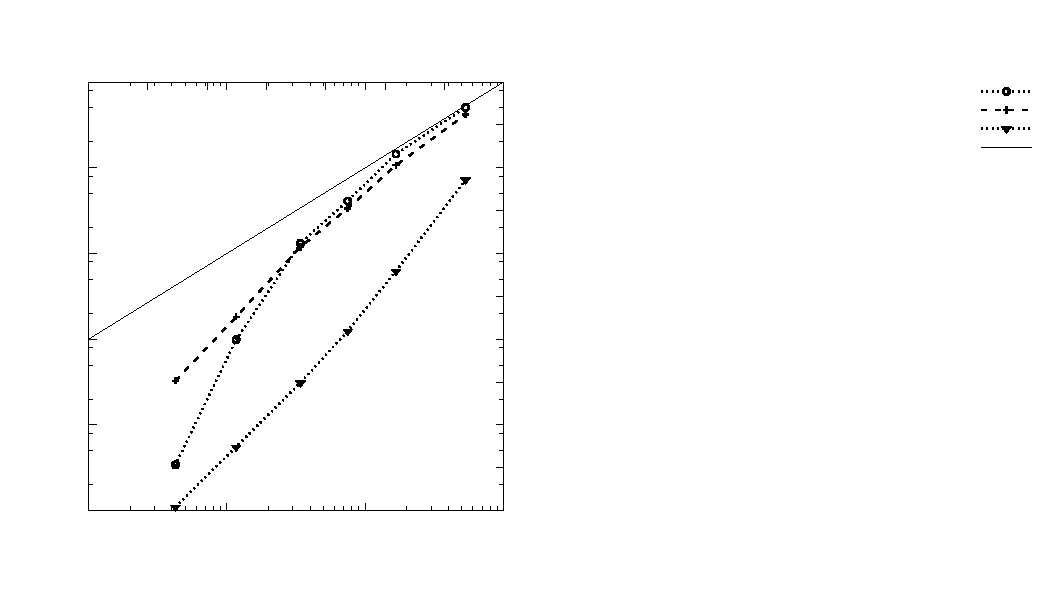
\includegraphics{NodePerformance}}%
    \gplfronttext
  \end{picture}%
\endgroup

	\end{center}
	\caption{
		Solver runtime vs. DoFs, for polynomial degree $k=2/1$,
		for problem/Equation (\ref{eq:NavierStokesCavityBenchmark}).
	}
	\label{fig:DrivenCavity}
\end{figure}